% =============================================================================
% NEMO-C manuscript -- IEEE Access format.
% Compile on Overleaf with the official "IEEE Access LaTeX template": copy this
% file and the figures/ folder into that project (it supplies ieeeaccess.cls and
% the logo files), then compile with pdfLaTeX.
% Every number in the results comes from results/results.csv and
% paper/paperdata.json; the plots are drawn by paper/make_figures.py.
% =============================================================================
\documentclass{ieeeaccess}
\usepackage{cite}
\usepackage{amsmath,amssymb,amsfonts}
\usepackage{algorithm}
\usepackage{algorithmic}
\usepackage{graphicx}
\usepackage{textcomp}
\usepackage{array}
\usepackage{url}
\usepackage{tikz}
\usetikzlibrary{arrows.meta,positioning,shapes.geometric,fit,calc}
\makeatletter
\ifdefined\pgfutil@addpdfresource@colorspaces
  \immediate\pdfobj{<</C0[0 0 0 0]/FunctionType 2/C1[1 0.3 0 0.2]/Domain[0 1]/N 1>>}
  \immediate\pdfobj{[/Separation/PANTONE3015C/DeviceCMYK \the\pdflastobj\space 0 R]}
  \edef\nemoc@pantone{/PANTONE3015C \the\pdflastobj\space 0 R}
  \expandafter\pgfutil@addpdfresource@colorspaces\expandafter{\nemoc@pantone}
\fi
\makeatother
\tikzset{
  blk/.style={draw, rounded corners=2pt, align=center, font=\scriptsize, minimum height=9mm, text width=#1, fill=white},
  blk/.default=24mm,
  dec/.style={draw, diamond, aspect=2.3, align=center, font=\scriptsize, inner sep=1pt, fill=white},
  arr/.style={-{Stealth[length=1.6mm]}, semithick},
  lbl/.style={font=\scriptsize, inner sep=1pt}
}

\begin{document}
\history{Manuscript submitted for BCSE307P Compiler Design, Vellore Institute of Technology, October 2026.}

\title{NEMO-C: Teaching a Compiler When \emph{Not} to Offload to Processing-in-Memory}

\author{\uppercase{Somesh Tripathi}\authorrefmark{1},
\uppercase{Smeehen}\authorrefmark{1},
\uppercase{Swati Saumya}\authorrefmark{1}}

\address[1]{School of Computer Science and Engineering, Vellore Institute of Technology, Vellore, Tamil Nadu 632014, India (Reg. Nos. 24BCE0533, 24BCE0502, 24BCE0253)}

\tfootnote{This work received no specific grant from any funding agency in the public, commercial, or not-for-profit sectors.}

\markboth
{Tripathi \headeretal: NEMO-C: Teaching a Compiler When Not to Offload to Processing-in-Memory}
{Tripathi \headeretal: NEMO-C: Teaching a Compiler When Not to Offload to Processing-in-Memory}

\corresp{Corresponding author: Somesh Tripathi (e-mail: somesh.tripathi2024@vitstudent.ac.in).}

\begin{abstract}
Processing-in-memory (PIM) places small processors inside DRAM so that data-intensive code can run where its data already lives, and commercial PIM devices are now available. Their programmers, however, must decide by hand which loops to move to the memory-side processors, and a wrong choice can make a program slower than running it on the CPU alone. Current PIM software stacks either leave this choice to the programmer through libraries and data-parallel interfaces, or make it inside domain-specific compilers for neural networks and in-DRAM bit-serial operations. None of them gives a general loop compiler a static, explainable rule that refuses an offload when the cost of moving data, launching the device and losing cache reuse outweighs the gain. We present NEMO-C, a compiler built from scratch in C++17 with Flex and Bison, that decides for every loop nest whether it should run on the host or on 64 DPUs. Its rule combines arithmetic intensity, data reuse, dependence-based parallelism, partitionability and a launch-cost size check, and loop fission, interchange and fusion turn some rejected loops into profitable ones. On 15 benchmarks in a cycle-level simulator, NEMO-C is never slower than the host, reaches a geometric-mean speedup of 1.42$\times$ (up to 7.47$\times$), and avoids the 0.63$\times$, 0.70$\times$ and 0.43$\times$ slowdowns that blind offloading causes; all 45 runs are bit-identical. Future work will calibrate the cost model on real UPMEM hardware and extend it to irregular and multi-kernel programs.
\end{abstract}

\begin{keywords}
Compiler optimization, cost model, data movement, dependence analysis, near-memory computing, processing-in-memory
\end{keywords}

\titlepgskip=-21pt

\maketitle

% =============================================================================
\section{Introduction}
\label{sec:introduction}
% =============================================================================

\PARstart{F}{or} many data-intensive programs the time spent moving data between main memory and the processor now outweighs the time spent computing on it. Mutlu \emph{et al.} argue that this movement is the dominant cost for a broad class of workloads and that computation should be performed where the data reside \cite{mutlu2019where}. Processing-in-memory (PIM) and the closely related near-memory computing (NMC) attach processing elements to, or place them inside, the memory modules so that streaming code does not have to cross the off-chip bus at all \cite{singh2019nmc, mutlu2020primer}. The idea is no longer only an academic one: UPMEM ships DDR4 modules in which every DRAM chip contains general-purpose in-order cores called DPUs \cite{devaux2019upmem}, and Samsung has built a function-in-memory HBM2 device with programmable compute units next to the banks \cite{kwon2021fimdram}.

Placing a processor next to memory does not by itself make a program faster. A loop sent to the DPUs has to pay for launching and synchronising the device, for copying its operands into the DPUs' small scratchpads, and for giving up the host's caches, which may already have been serving most of its accesses \cite{ghose2019workload}. A loop that does a lot of arithmetic per byte, that re-reads its data, or whose iterations need data owned by other DPUs, can therefore run more slowly in memory than on the CPU. Studies of consumer-device and general-purpose workloads confirm that the benefit depends strongly on the kind of bottleneck a function exhibits \cite{boroumand2018google, oliveira2022methodologies}. Today the programmer of a PIM system has to make this call for every kernel, by hand. The problem we address is to make the call automatically, at compile time, and to make it correctly in both directions: offload the loops that gain, and refuse the ones that lose.

Two families of existing work bear on this problem. The first characterises real PIM hardware and gives programmers practical guidance. Benchmark studies of the UPMEM system, and evaluations of machine-learning and transcendental-function workloads on it, show which kinds of kernels suit DPUs and which do not \cite{gomezluna2023ml, item2023transpimlib}. Industry prototypes report large gains for the memory-bound parts of recommendation and neural-network inference when those parts are chosen carefully \cite{ke2020recnmp, kwon2021fimdram}.

The second family builds programming support around PIM: libraries, data-parallel frameworks and domain-specific compilers that generate PIM code from a higher-level description. These tools reduce the effort of writing PIM code considerably. Classical compiler technology supplies the remaining ingredients, namely dependence analysis, loop transformations, dataflow analysis and register allocation, all of which are mature and well documented \cite{cooper2022engineering}. Section~\ref{sec:related} reviews fifteen recent systems of both kinds in detail \cite{gomezluna2022prim, devic2022topim, khan2023cinm, chen2023simplepim, oliveira2023dappa, shin2023pimflow, oliveira2021damov, giannoula2022sparsep, boroumand2019conda, wang2023infinity, oliveira2024mimdram, hajinazar2021simdram, lee2021hbmpim, hyun2024pathfinding, sun2023pimcomp}.

The shortfall of the first family is that its knowledge stays in papers and in programmers' heads. A characterisation study can say that kernels with heavy inter-DPU communication scale poorly, but nothing in the tool chain applies that observation to a new loop. The programmer still decides, still has to estimate data movement by hand, and receives no warning when an offload is unprofitable.

The shortfall of the second family is that most of its tools assume the decision has already been made. A library or a data-parallel framework generates efficient PIM code for whatever the programmer marks for PIM; a neural-network compiler maps layers that are known in advance to suit the device. Few of them combine a static cost model with dependence analysis for general loop nests, few of them use loop transformations to make a rejected loop profitable, and few explain their decision in terms a programmer can check. Among the tools we reviewed, only the framework of Devic \emph{et al.} treats refusing an offload as a first-class outcome, and none pairs that refusal with loop transformations that make the loop profitable instead.

This paper proposes NEMO-C (a NEar-Memory-aware Optimising Compiler), which closes this gap for affine loop programs. For every loop nest, NEMO-C computes five classical properties: arithmetic intensity, self-temporal reuse weighted by its share of the traffic, parallelism from GCD and Banerjee dependence tests, partitionability under the owner-computes rule, and an estimate of whether the nest is large enough to pay for launching the DPUs. It offloads the nest only if all checks pass. When a nest fails, loop fission, interchange and fusion are tried, and the nest is decided again. Offloaded nests are partitioned across 64 DPUs, flush and invalidate operations are placed by a forward dataflow analysis, and DPU assembly is generated with scratchpad tiling and Chaitin--Briggs graph-colouring register allocation.

The approach suits the problem because each check corresponds to a concrete reason why offloading can fail, and each is computed by an analysis whose correctness is well understood. The decision is static, so it needs neither hardware nor profiling runs, and it is explainable: the compiler prints every number and every check behind a verdict. The advantage shows in the results. Across 15 benchmarks NEMO-C is never slower than the host, while blind offloading loses on four of them, and a single-metric rule based on arithmetic intensity loses on three. Every configuration of every benchmark produces bit-identical results, including runs that execute the generated DPU assembly itself.

The rest of the paper is organised as follows. Section~\ref{sec:related} reviews fifteen related systems and the gap each leaves. Section~\ref{sec:proposed} formulates the problem and presents the architecture, modules, equations and algorithms of NEMO-C. Section~\ref{sec:results} describes the implementation, the experimental setup and the results for six metrics, and compares NEMO-C with three related works. Section~\ref{sec:conclusion} concludes and outlines future work.

% =============================================================================
\section{Related Works}
\label{sec:related}
% =============================================================================

This section reviews fifteen recent works on PIM characterisation, programming support, compilation and hardware. For each we summarise the solution, the methodology and tools, the reported results, and the research gap relative to automatic offload decisions for general loop programs. Table~\ref{tab:related} summarises them.

\subsection{Experimental Characterisation of a Real PIM System (PrIM)}
\textbf{Solution.} G\'omez-Luna \emph{et al.} present the first comprehensive experimental analysis of the publicly available UPMEM PIM architecture, in which DRAM arrays and in-order DPU cores share the same chip \cite{gomezluna2022prim}. Their aim is to tell programmers and architects what the hardware can and cannot do well.

\textbf{Methodology and tools.} The study first measures the limits of the hardware with microbenchmarks that isolate the DPUs' compute throughput and the bandwidth of their local memory and of host--DPU transfers. These measurements expose, for example, how arithmetic throughput depends on the operation and data type, and how the scratchpad and the DRAM bank behave under different access patterns.

The authors then introduce PrIM, a suite of 16 memory-bound workloads drawn from linear algebra, databases, graph processing, neural networks and other domains, and port each one by hand to UPMEM. The workloads were run on two UPMEM systems with 640 and 2,556 DPUs, and their scaling and performance were compared with conventional processors.

\textbf{Results.} The study finds that workloads with streaming access, little or no inter-DPU communication and simple arithmetic benefit most, while workloads that need frequent communication between DPUs, which on UPMEM must pass through the host, scale poorly.

\textbf{Research gap.} The guidance is empirical and is applied by hand; no compiler applies it automatically to a new loop.

\subsection{To PIM or Not for General-Purpose Processing in DDR Systems}
\textbf{Solution.} Devic \emph{et al.} study PIM hardware that places a general-purpose RISC-V core at each memory bank, and present a software compilation framework that decides what, whether, when and how to offload work to these bank-level engines \cite{devic2022topim}. They also propose a vector-engine extension to the bank cores.

\textbf{Methodology and tools.} The framework starts from off-the-shelf C/C++ applications and identifies regions that could execute on the bank-level cores. It then decides, region by region, whether offloading is worthwhile, which makes the work one of the few to treat offloading as a decision rather than a default.

The evaluation is simulation-based; the authors' public repository (BLIMP, Bank-Level In-memory Processing) provides the benchmarks, the instrumentation, the compilation flow and the simulation setup. They also study how the number of memory banks and the relative speed of host and PIM cores change the answer.

\textbf{Results.} The authors report that PIM is not always beneficial for off-the-shelf applications, so selective offloading matters, and that bank count and core speeds shift the to-PIM-or-not decision.

\textbf{Research gap.} The work targets bank-level RISC-V cores and whole application regions; loop-level enabling transformations and a per-loop explanation of each verdict are outside its stated scope.

\subsection{CINM: A Compilation Infrastructure for In- and Near-Memory Computing}
\textbf{Solution.} Khan \emph{et al.} present Cinnamon (CINM), an end-to-end compilation flow that targets both compute-in-memory (CIM) devices, such as memristive crossbars, and compute-near-memory (CNM) devices, such as UPMEM, from one program representation \cite{khan2023cinm}. They argue that existing programming models are too low-level and too tied to a particular system.

\textbf{Methodology and tools.} CINM uses hierarchical abstractions: a program is lowered progressively from a device-independent representation to device-specific ones, and optimisations are applied at each level of the lowering pipeline. This lets common optimisations be shared across devices while device-specific ones are applied late.

The evaluation compiles a set of benchmarks for a real CNM system (UPMEM) and for memristor-based CIM accelerators, and compares the generated code with state-of-the-art hand-written implementations.

\textbf{Results.} The authors report that the generated code is comparable to, or better than, the state-of-the-art implementations.

\textbf{Research gap.} CINM generates code for kernels that are mapped to the in-memory device; it does not decide, from a cost model, that a kernel should stay on the host.

\subsection{SimplePIM: A Software Framework for Productive PIM Programming}
\textbf{Solution.} Chen \emph{et al.} propose SimplePIM, a high-level framework that lets the host drive PIM devices through iterator functions over arrays (such as map and reduce) and supplies communication primitives between the host and the PIM cores \cite{chen2023simplepim}.

\textbf{Methodology and tools.} The programmer expresses a computation as array iterators with user-defined element functions; SimplePIM handles the distribution of data, the launching of the DPUs and the gathering of results. Its interface handles arrays of arbitrary element types.

The framework is implemented on the UPMEM system and evaluated on six applications, including vector addition, reduction, histogram, K-means clustering and linear and logistic regression, against hand-optimised UPMEM baselines.

\textbf{Results.} SimplePIM reduces lines of code by 66.5\% to 83.1\% and achieves speedups of 10\% to 37\% over hand-optimised code in three applications, with comparable performance in the other three.

\textbf{Research gap.} The programmer still chooses what runs on PIM; the framework does not reject an unprofitable offload.

\subsection{DaPPA: A Data-Parallel Programming Framework for PIM}
\textbf{Solution.} Oliveira \emph{et al.} propose DaPPA, a framework that hides UPMEM's explicit data management and workload partitioning behind data-parallel patterns \cite{oliveira2023dappa}.

\textbf{Methodology and tools.} DaPPA has three parts: a set of five data-parallel pattern primitives, a dataflow programming interface that lets patterns be composed, and a dynamic template-based compiler that turns the description into an optimised UPMEM binary. Memory allocation, data distribution and gathering, and parallelisation are handled automatically.

It is evaluated on six workloads from the PrIM suite on a real UPMEM system and compared with the hand-tuned PrIM implementations in performance and in programming effort.

\textbf{Results.} DaPPA improves end-to-end performance by 2.1$\times$ on average over the hand-tuned versions and reduces lines of code by 94\% on average.

\textbf{Research gap.} Like SimplePIM, it optimises code that the programmer has already decided to run on PIM.

\subsection{PIMFlow: Compiler and Runtime Support for CNNs on DRAM-PIM}
\textbf{Solution.} Shin \emph{et al.} present PIMFlow, an end-to-end compiler and runtime that runs convolutional neural networks on a GPU whose memory contains DRAM-PIM units \cite{shin2023pimflow}. They observe that recent CNNs increasingly use computationally lightweight layers, which suit PIM.

\textbf{Methodology and tools.} PIMFlow transforms the model graph to create parallelism between nodes so that some layers can run on the GPU and others on PIM at the same time, and it explores task-parallel and data-parallel execution scenarios to minimise execution time.

It provides a code-generating back end and an execution engine for DRAM-PIM, and it is integrated with the TVM compiler for the graph-level optimisations.

\textbf{Results.} PIMFlow achieves up to 82\% end-to-end speedup and an average 26\% energy reduction for CNN inference.

\textbf{Research gap.} The decision is made for neural-network layers inside a GPU system; general affine loop nests on a host CPU are not addressed.

\subsection{DAMOV: Classifying Data-Movement Bottlenecks}
\textbf{Solution.} Oliveira \emph{et al.} present DAMOV, a methodology and benchmark suite for finding the sources of data-movement bottlenecks and choosing the right mitigation for them, with near-data processing as the main case study \cite{oliveira2021damov}.

\textbf{Methodology and tools.} The methodology has three steps and uses four key metrics to classify each function into one of six classes of memory bottleneck. It was applied to 77K functions from 345 applications.

From this characterisation the authors select 144 functions as the open-source DAMOV suite and use the classification to decide which mitigation mechanism, such as near-data processing, suits each class.

\textbf{Results.} The study shows that the right mitigation depends on the bottleneck class, and it releases the suite and tool chain for further studies.

\textbf{Research gap.} The classification is an offline profiling study; it is not embedded in a compiler that acts on it per loop.

\subsection{SparseP: Sparse Matrix--Vector Multiplication on Real PIM}
\textbf{Solution.} Giannoula \emph{et al.} present SparseP, the first library of sparse matrix--vector multiplication (SpMV) kernels for real PIM systems, together with the first analysis of SpMV on such hardware \cite{giannoula2022sparsep}.

\textbf{Methodology and tools.} SparseP provides 25 SpMV kernels across four compressed formats (CSR, COO, BCSR and BCOO) and several schemes for partitioning the matrix and balancing load across DPUs.

The kernels are evaluated on a real UPMEM system with 2,528 PIM cores and compared with CPU and GPU systems in performance and energy.

\textbf{Results.} The study identifies how partitioning and load balancing decide whether this irregular, memory-bound kernel benefits from PIM.

\textbf{Research gap.} The library hand-optimises one kernel; it does not provide a general rule for other loops.

\subsection{CoNDA: Cache Coherence for Near-Data Accelerators}
\textbf{Solution.} Boroumand \emph{et al.} propose CoNDA, a coherence mechanism for near-data accelerators (NDAs) that sit off-chip near main memory \cite{boroumand2019conda}. They find that existing coherence mechanisms erase most of the benefit of NDAs.

\textbf{Methodology and tools.} CoNDA lets the NDA execute a kernel optimistically, as if it already held the needed coherence permissions. It records the memory accesses of the NDA and of the rest of the system during the kernel and resolves conflicts afterwards, skipping coherence requests that turn out to be unnecessary.

It is evaluated on graph-processing and hybrid in-memory database workloads and compared with prior coherence mechanisms and with an ideal, zero-cost mechanism.

\textbf{Results.} CoNDA improves performance by 19.6\% over the best prior mechanism on modest data sets (38.3\% on large ones) and comes within 10.4\% of the ideal mechanism.

\textbf{Research gap.} CoNDA is a hardware mechanism; a compiler that knows which arrays a kernel reads and writes can place the needed flushes and invalidations statically.

\subsection{Infinity Stream: In-/Near-Memory Fusion}
\textbf{Solution.} Wang \emph{et al.} present Infinity Stream, which combines in-memory computing in large last-level caches with near-memory computing in a portable and programmer-friendly way \cite{wang2023infinity}.

\textbf{Methodology and tools.} The work introduces a tensor dataflow graph (tDFG) as an intermediate representation that captures both in-memory and near-memory computation. A two-phase, JIT-based compilation lowers the tDFG to in-memory commands, which keeps programs portable across microarchitectures.

It addresses automatic parallelisation, data transposition for bit-serial logic and the combination of in- and near-memory computing, and it is evaluated with a cycle-accurate simulator on fp32 data-processing workloads.

\textbf{Results.} Infinity Stream reports a 2.6$\times$ speedup, a 75\% traffic reduction and 2.4$\times$ energy efficiency over a state-of-the-art near-memory technique.

\textbf{Research gap.} It targets cache-resident bit-serial computation, not near-bank DPUs, and its scope is the mapping of computation rather than a refusal rule.

\subsection{MIMDRAM: MIMD Processing-Using-DRAM}
\textbf{Solution.} Oliveira \emph{et al.} present MIMDRAM, an end-to-end processing-using-DRAM (PUD) system that exploits fine-grained DRAM to run multiple instruction streams in each DRAM subarray \cite{oliveira2024mimdram}.

\textbf{Methodology and tools.} Because smaller segments of a wide DRAM row can be activated independently, MIMDRAM executes MIMD operations across segments, with SIMD inside each segment, which uses the DRAM array more efficiently than whole-row SIMD.

Its compiler passes take unmodified C/C++ code, identify loops suitable for PUD execution, transform them to use PUD operations, and schedule independent operations to run concurrently.

\textbf{Results.} MIMDRAM reports 34$\times$ the performance, 14.3$\times$ the energy efficiency, 1.7$\times$ the throughput and 1.3$\times$ the fairness of a state-of-the-art PUD framework, with an area overhead of 1.11\% of a DRAM chip and 0.6\% of a CPU die.

\textbf{Research gap.} Its loop selection is for bit-serial in-DRAM execution, not for near-bank cores that pay launch and DMA costs.

\subsection{SIMDRAM: Bit-Serial SIMD Processing Using DRAM}
\textbf{Solution.} Hajinazar \emph{et al.} present SIMDRAM, a flexible, general-purpose processing-using-DRAM framework that uses each DRAM column as an independent SIMD lane for bit-serial operations \cite{hajinazar2021simdram}.

\textbf{Methodology and tools.} SIMDRAM works in three steps: it builds an efficient representation of a desired operation using majority (MAJ) and NOT logic, maps the operands and the operation onto DRAM rows and commands, and executes the operation.

The framework is evaluated against a state-of-the-art in-DRAM computing mechanism and against a CPU and a high-end GPU.

\textbf{Results.} SIMDRAM provides up to 5.1$\times$ higher operation throughput and 2.5$\times$ higher energy efficiency than the prior in-DRAM mechanism, with less than 1\% DRAM chip area overhead, and is 257$\times$ and 31$\times$ more energy-efficient than the CPU and GPU.

\textbf{Research gap.} It provides operations for in-DRAM execution but leaves the choice between host and memory to the programmer.

\subsection{HBM-PIM: Architecture and Software Stack on Commercial DRAM}
\textbf{Solution.} Lee \emph{et al.} present a PIM architecture built on commercial HBM2 DRAM, with a lightweight PIM unit at the I/O boundary between the DRAM cells and the peripheral circuitry, shared by each pair of banks \cite{lee2021hbmpim}.

\textbf{Methodology and tools.} The device is implemented in a 20\,nm DRAM technology and integrated with an unmodified commercial processor; host column read and write commands are reused to trigger PIM execution, which keeps it compatible with JEDEC memory controllers.

The authors developed the software stack needed to run existing applications without changing their source code and evaluated it on memory-bound neural-network kernels and full applications.

\textbf{Results.} PIM improves memory-bound neural-network kernels by 11.2$\times$ and applications by 3.5$\times$, and reduces energy per bit transferred by 3.5$\times$.

\textbf{Research gap.} The stack offloads operations known to be memory-bound in machine learning; general loop nests and the decision to refuse offloading are not addressed.

\subsection{Pathfinding Future PIM Architectures (uPIMulator)}
\textbf{Solution.} Hyun \emph{et al.} demystify UPMEM's commercial PIM technology and use the insight to identify features that future PIM architectures will need \cite{hyun2024pathfinding}.

\textbf{Methodology and tools.} They built uPIMulator, which compiles UPMEM-PIM source code into machine-level instructions and feeds them to a cycle-level performance simulator.

With the simulator they characterise the UPMEM design in detail and run case studies on possible architectural changes.

\textbf{Results.} The work provides a validated simulation infrastructure and a set of architectural directions for general-purpose PIM.

\textbf{Research gap.} It is an architecture-exploration tool; deciding which code to offload is left to the programmer.

\subsection{PIMCOMP: A Compilation Framework for Crossbar-Based PIM}
\textbf{Solution.} Sun \emph{et al.} present PIMCOMP, a universal compilation framework for non-volatile-memory crossbar-based PIM accelerators for deep neural networks \cite{sun2023pimcomp}.

\textbf{Methodology and tools.} PIMCOMP is built on an abstract accelerator model that matches the common crossbar, in-memory-accelerator, tile and chip hierarchy. Its compiler runs four stages: node partitioning, weight replication, core mapping and dataflow scheduling.

It offers two modes with different inter-layer pipeline granularities, one for high throughput and one for low latency, and is compared with the PUMA compiler.

\textbf{Results.} PIMCOMP reports 1.6$\times$ higher throughput and 2.4$\times$ lower latency than PUMA.

\textbf{Research gap.} It targets DNN layers on crossbars; general loop nests and host-versus-PIM profitability are outside its scope.

\begin{table*}[!t]
\caption{Summary of related work and the gap each leaves for automatic offload decisions on general loop programs.}
\label{tab:related}
\setlength{\tabcolsep}{4pt}
\renewcommand{\arraystretch}{1.12}
\centering
\begin{tabular}{|p{2.6cm}|p{4.2cm}|p{3.2cm}|p{6.6cm}|}
\hline
\textbf{Work} & \textbf{Approach} & \textbf{Platform} & \textbf{Gap relative to NEMO-C} \\ \hline
PrIM \cite{gomezluna2022prim} & Microbenchmarks and 16 hand-ported workloads & Real UPMEM (640, 2,556 DPUs) & Guidance applied by hand, no automatic decision \\ \hline
Devic \emph{et al.} \cite{devic2022topim} & Compilation framework deciding what and whether to offload & Simulated RISC-V core per bank & Region level; no loop transformations or per-loop explanation reported \\ \hline
CINM \cite{khan2023cinm} & Hierarchical progressive lowering & UPMEM and memristive CIM & Compiles mapped kernels; no refusal rule \\ \hline
SimplePIM \cite{chen2023simplepim} & Host-driven array iterators & Real UPMEM & Programmer chooses offloads \\ \hline
DaPPA \cite{oliveira2023dappa} & Data-parallel patterns, template compiler & Real UPMEM & Programmer chooses offloads \\ \hline
PIMFlow \cite{shin2023pimflow} & CNN graph transforms, TVM integration & GPU with DRAM-PIM & CNN layers only \\ \hline
DAMOV \cite{oliveira2021damov} & Bottleneck classification of 77K functions & Profiling and simulation & Offline study, not in a compiler \\ \hline
SparseP \cite{giannoula2022sparsep} & 25 SpMV kernels, 4 formats & Real UPMEM (2,528 cores) & One hand-optimised kernel \\ \hline
CoNDA \cite{boroumand2019conda} & Optimistic hardware coherence & Simulated NDA & Hardware; no static placement \\ \hline
Infinity Stream \cite{wang2023infinity} & tDFG IR, JIT lowering & Simulated LLC in-memory & Cache bit-serial; no refusal rule \\ \hline
MIMDRAM \cite{oliveira2024mimdram} & Fine-grained MIMD PUD, compiler passes & Simulated DRAM & Bit-serial PUD, not near-bank cores \\ \hline
SIMDRAM \cite{hajinazar2021simdram} & MAJ/NOT bit-serial framework & Simulated DRAM & Programmer chooses offloads \\ \hline
HBM-PIM \cite{lee2021hbmpim} & PIM units at bank I/O, software stack & Real HBM2 prototype & ML operations only \\ \hline
uPIMulator \cite{hyun2024pathfinding} & Compiler and cycle-level simulator & Simulated UPMEM & Architecture exploration only \\ \hline
PIMCOMP \cite{sun2023pimcomp} & Four-stage DNN mapping & Crossbar NVM PIM & DNN-specific \\ \hline
\textbf{NEMO-C (this work)} & \textbf{Six-check static cost model with dependence analysis and enabling transformations} & \textbf{Cycle-level UPMEM-style model} & \textbf{Decides per loop nest, refuses unprofitable offloads, explains each verdict} \\ \hline
\end{tabular}
\end{table*}

% =============================================================================
\section{Proposed System}
\label{sec:proposed}
% =============================================================================

\subsection{Problem Formulation}
\label{sec:formulation}

A program is a sequence of host blocks and kernels over multidimensional arrays; every kernel is a list of loop nests $\mathcal{L}=\{L_1,\dots,L_m\}$ whose loop bounds are compile-time constants. The target machine has a host CPU with a cache and $P=64$ DPUs, each with a private DRAM bank and a 64\,KB scratchpad (WRAM). DPUs cannot exchange data directly; anything one DPU needs from another must pass through the host. The compiler must choose a mapping $M:\mathcal{L}\rightarrow\{\textsc{host},\textsc{dpu}\}$ and generate code for it. The mapping must not change the program's results, and it should minimise total execution time.

We ask for more than a low average time. A mapping is acceptable only if no nest is offloaded when offloading makes it slower; formally, for every nest, $T(L,M(L))\le T(L,\textsc{host})$. The decision must be made at compile time from static analysis alone, without hardware, profiling runs or input data. The cost of a nest on the DPUs is not known exactly at compile time, so the compiler must reason with conservative estimates and must be able to explain each verdict. When a nest is rejected, the compiler may apply semantics-preserving loop transformations and decide again.

\subsection{System Architecture}
\label{sec:architecture}

Fig.~\ref{fig:arch} shows the architecture of NEMO-C. It is organised as nine phases, labelled A to I, which follow the classical front end, middle end and back end of a compiler and add a simulator for validation. The front end (A) scans the \texttt{.nmc} source with a Flex-generated DFA, parses it with a Bison-generated LALR(1) parser that has no grammar conflicts, and checks it semantically against a scoped symbol table. The middle end lowers the tree to three-address code that keeps loop nests intact and builds a control-flow graph on demand (B), runs five classical optimisations (C) and computes access matrices, dependences and parallel loops (D).

The decision phase (E) is the centre of the design. It receives the dependence information and the IR of each nest and either accepts the nest for the DPUs or rejects it; a rejected nest is passed to the transformation phase (F), and the result is decided again. Accepted nests are partitioned across the DPUs and given coherence operations (G), after which the back end (H) generates DPU assembly with scratchpad tiling and graph-colouring register allocation, together with host C code that moves data and launches the DPUs. Rejected nests remain ordinary host code. Finally the simulator (I) runs the program three ways, checks that all results are bit-identical, executes the generated DPU assembly and reports cycles, memory-bus bytes and energy.

\begin{figure*}[!t]
\centering
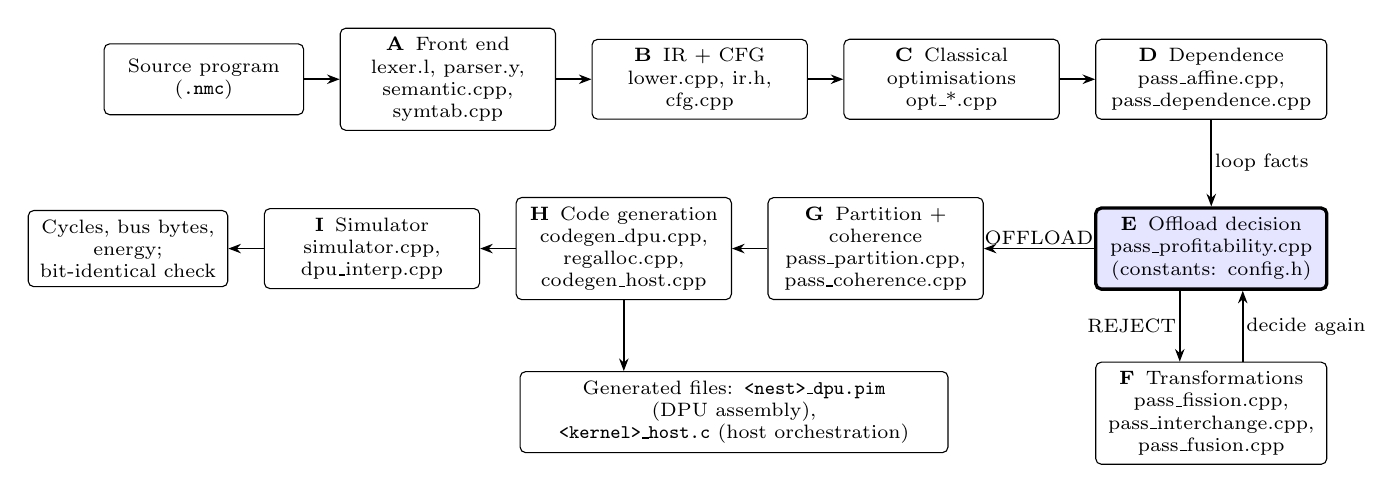
\begin{tikzpicture}[node distance=5mm and 4.5mm]
\node[blk=23mm] (src) {Source program\\(\texttt{.nmc})};
\node[blk=25mm, right=of src] (fe) {\textbf{A}\enspace Front end\\lexer.l, parser.y,\\semantic.cpp, symtab.cpp};
\node[blk=25mm, right=of fe] (ir) {\textbf{B}\enspace IR + CFG\\lower.cpp, ir.h,\\cfg.cpp};
\node[blk=25mm, right=of ir] (opt) {\textbf{C}\enspace Classical\\optimisations\\opt\_*.cpp};
\node[blk=27mm, right=of opt] (dep) {\textbf{D}\enspace Dependence\\pass\_affine.cpp,\\pass\_dependence.cpp};
\node[blk=27mm, below=11mm of dep, fill=blue!10, very thick] (dec) {\textbf{E}\enspace Offload decision\\pass\_profitability.cpp\\(constants: config.h)};
\node[blk=25mm, left=14mm of dec] (part) {\textbf{G}\enspace Partition +\\coherence\\pass\_partition.cpp,\\pass\_coherence.cpp};
\node[blk=25mm, left=of part] (cg) {\textbf{H}\enspace Code generation\\codegen\_dpu.cpp,\\regalloc.cpp,\\codegen\_host.cpp};
\node[blk=25mm, left=of cg] (sim) {\textbf{I}\enspace Simulator\\simulator.cpp,\\dpu\_interp.cpp};
\node[blk=23mm, left=of sim] (out) {Cycles, bus bytes,\\energy;\\bit-identical check};
\node[blk=27mm, below=9mm of dec] (tr) {\textbf{F}\enspace Transformations\\pass\_fission.cpp,\\pass\_interchange.cpp,\\pass\_fusion.cpp};
\node[blk=52mm, below=9mm of cg, xshift=14mm] (files) {Generated files: \texttt{<nest>\_dpu.pim} (DPU assembly),\\\texttt{<kernel>\_host.c} (host orchestration)};
\draw[arr] (src) -- (fe);
\draw[arr] (fe) -- (ir);
\draw[arr] (ir) -- (opt);
\draw[arr] (opt) -- (dep);
\draw[arr] (dep) -- node[lbl, right] {loop facts} (dec);
\draw[arr] (dec) -- node[lbl, above] {OFFLOAD} (part);
\draw[arr] (part) -- (cg);
\draw[arr] (cg) -- (sim);
\draw[arr] (sim) -- (out);
\draw[arr] ([xshift=-4mm]dec.south) -- node[lbl, left] {REJECT} ([xshift=-4mm]tr.north);
\draw[arr] ([xshift=4mm]tr.north) -- node[lbl, right] {decide again} ([xshift=4mm]dec.south);
\draw[arr] (cg.south) -- ([xshift=-14mm]files.north);
\end{tikzpicture}
\caption{Architecture of NEMO-C. Phases A--D analyse the program, phase E decides for every loop nest whether it runs on the host or the DPUs, phase F rewrites rejected nests so they can be decided again, and phases G--I generate, partition and validate the code. Rejected nests stay in the host code.}
\label{fig:arch}
\end{figure*}

\subsection{Modules and Their Functions}
\label{sec:modules}

Table~\ref{tab:modules} lists the modules. The compiler consists of 43 source files and about 11,400 lines of C++17, Flex and Bison, with one file per pass so that each analysis can be tested and explained in isolation; each file begins with a comment naming the compiler-theory concept and the standard algorithm it implements. A separate test suite of eight programs with 365 checks exercises every pass, and a browser-based workbench (\texttt{web/server.py}) runs the same compiler on any program for demonstration.

\begin{table}[!t]
\caption{Modules of NEMO-C and their functions.}
\label{tab:modules}
\setlength{\tabcolsep}{3pt}
\renewcommand{\arraystretch}{1.1}
\centering
\begin{tabular}{|p{0.5cm}|p{2.6cm}|p{4.7cm}|}
\hline
\textbf{Ph.} & \textbf{Module (files)} & \textbf{Function} \\ \hline
A & lexer.l & DFA scanner, maximal munch, line and column tracking \\ \hline
A & parser.y, ast.cpp & LALR(1) parser, 0 conflicts, panic-mode recovery, AST \\ \hline
A & symtab.cpp, semantic.cpp & Scoped symbol table; type, bound and loop-index checks \\ \hline
B & lower.cpp, ir.h, cfg.cpp & Three-address IR with nested loops; CFG on demand \\ \hline
C & opt\_constfold, opt\_cse, opt\_dce, opt\_indvar, opt\_strength & Constant propagation, CSE, dead-code elimination, induction variables, strength reduction \\ \hline
D & pass\_affine, pass\_dependence & Access matrices; GCD and Banerjee tests; direction vectors; reductions \\ \hline
E & pass\_profitability & Six-check offload decision and plain-English trace \\ \hline
F & pass\_fission, pass\_interchange, pass\_fusion & Allen--Kennedy fission, loop interchange, loop fusion \\ \hline
G & pass\_partition, pass\_coherence & Owner-computes partitioning; flush/invalidate placement \\ \hline
H & codegen\_dpu, regalloc, codegen\_host & PIM assembly with tiling; Chaitin--Briggs allocation; host C \\ \hline
I & simulator, dpu\_interp & Cycle, byte and energy model; execution of the generated DPU code \\ \hline
\end{tabular}
\end{table}

\subsection{Flow Diagram}
\label{sec:flow}

Fig.~\ref{fig:flow} shows how one program travels through the compiler. After parsing and checking, any error is reported with its file, line and column, and the parser recovers at the next statement so that all errors are reported in one run. A correct program is lowered and optimised, and then every loop nest is analysed and decided on its own. A nest that passes is partitioned and compiled for the DPUs. A nest that fails is offered to the transformations; if one applies, the transformed nests are decided again, otherwise the nest stays on the host. The simulator closes the loop by checking that the program computes exactly what the host-only program computes.

\begin{figure}[!t]
\centering
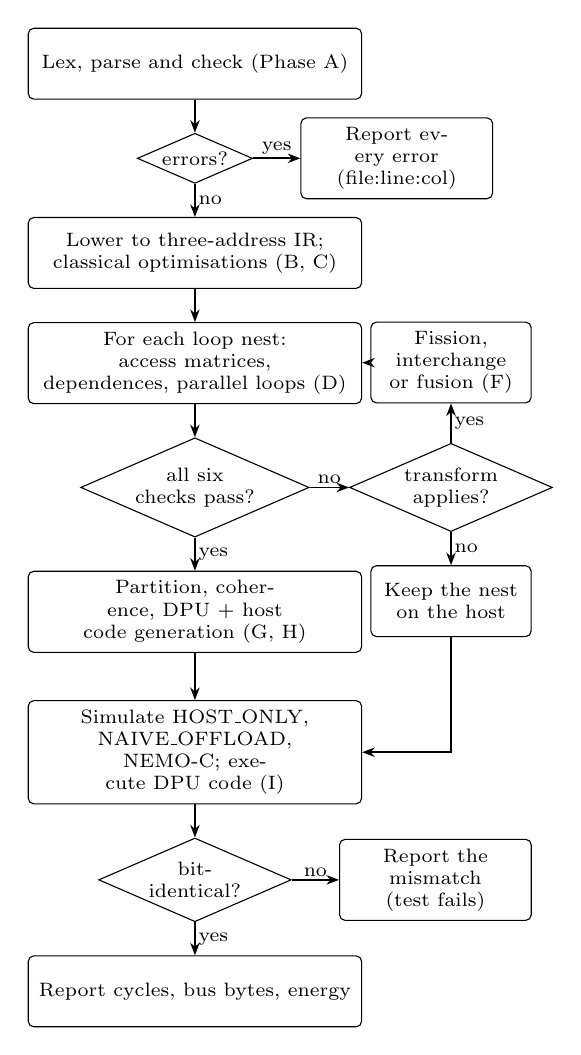
\begin{tikzpicture}[node distance=4.2mm]
\node[blk=40mm] (s1) {Lex, parse and check (Phase A)};
\node[dec, below=of s1] (d1) {errors?};
\node[blk=22mm, right=6mm of d1] (e1) {Report every error\\(file:line:col)};
\node[blk=40mm, below=of d1] (s2) {Lower to three-address IR;\\classical optimisations (B, C)};
\node[blk=40mm, below=of s2] (s3) {For each loop nest: access matrices,\\dependences, parallel loops (D)};
\node[dec, below=of s3] (d2) {all six\\checks pass?};
\node[dec, right=5mm of d2] (d3) {transform\\applies?};
\node[blk=18mm, above=5mm of d3] (t1) {Fission, interchange\\or fusion (F)};
\node[blk=40mm, below=of d2] (s4) {Partition, coherence, DPU + host\\code generation (G, H)};
\node[blk=18mm, below=of d3] (h1) {Keep the nest\\on the host};
\node[blk=40mm, below=6mm of s4] (s5) {Simulate HOST\_ONLY, NAIVE\_OFFLOAD,\\NEMO-C; execute DPU code (I)};
\node[dec, below=of s5] (d4) {bit-\\identical?};
\node[blk=22mm, right=6mm of d4] (e2) {Report the mismatch\\(test fails)};
\node[blk=40mm, below=of d4] (s6) {Report cycles, bus bytes, energy};
\draw[arr] (s1) -- (d1);
\draw[arr] (d1) -- node[lbl, above] {yes} (e1);
\draw[arr] (d1) -- node[lbl, right] {no} (s2);
\draw[arr] (s2) -- (s3);
\draw[arr] (s3) -- (d2);
\draw[arr] (d2) -- node[lbl, above] {no} (d3);
\draw[arr] (d3) -- node[lbl, right] {yes} (t1);
\draw[arr] (t1) -- (s3);
\draw[arr] (d3) -- node[lbl, right] {no} (h1);
\draw[arr] (d2) -- node[lbl, right] {yes} (s4);
\draw[arr] (h1.south) |- (s5.east);
\draw[arr] (s4) -- (s5);
\draw[arr] (s5) -- (d4);
\draw[arr] (d4) -- node[lbl, above] {no} (e2);
\draw[arr] (d4) -- node[lbl, right] {yes} (s6);
\end{tikzpicture}
\caption{Flow of a program through NEMO-C. Every loop nest is decided on its own; a rejected nest may be transformed and decided again, and the simulator checks that the final program is bit-identical to the host-only one.}
\label{fig:flow}
\end{figure}

\subsection{Detailed Methodology}
\label{sec:method}

\subsubsection{Front End and Intermediate Representation}
The source language has array and scalar declarations, \texttt{kernel} blocks that may be offloaded and \texttt{host} blocks that always run on the CPU, \texttt{for} loops with constant bounds and a positive step, \texttt{if}/\texttt{else}, assignment, \texttt{call} and \texttt{print}. The grammar is LALR(1) with zero shift/reduce and reduce/reduce conflicts; braces are mandatory on both arms of an \texttt{if}, so the dangling-else ambiguity cannot arise, and operator precedence is declared explicitly. The rule \texttt{stmt : error ';'} gives panic-mode recovery. The semantic pass checks that names are declared, that subscripts match the declared dimensions, that loop bounds are integer constants, that a loop index is not reassigned in its body, and that \texttt{print} and \texttt{call} appear only in host code, a context-sensitive rule that the context-free grammar cannot express.

Lowering produces three-address code in which every statement performs one load, store, operation or copy, with temporaries \texttt{\%t0}, \texttt{\%t1}, and so on. Unlike a textbook compiler, NEMO-C keeps loops and conditionals structured in the IR, because dependence analysis, the cost model and the loop transformations all need to see whole loop nests. A flat control-flow graph is built from the same IR whenever a dataflow pass needs one. Five classical passes then run in a fixed order: constant propagation over the lattice \{UNDEF, CONST, NAC\}, local common-subexpression elimination using available expressions, dead-code elimination driven by backward liveness, induction-variable recognition, and strength reduction that replaces $i\cdot c$ by an accumulator incremented by $c$. The last matters for PIM because a DPU multiply costs 16 cycles and an addition 2.

\subsubsection{Dependence Analysis}
Every array reference in a nest of depth $n$ is written in affine form
\begin{equation}
f(\mathbf{i}) = F\,\mathbf{i} + \mathbf{c},
\label{eq:affine}
\end{equation}
where $\mathbf{i}=(i_1,\dots,i_n)^{\top}$ is the vector of loop indices, $F$ is the integer access matrix with one row per array dimension and one column per loop, and $\mathbf{c}$ is the offset vector. For \texttt{A[2i+1]}, $F=(2)$ and $\mathbf{c}=(1)$. A subscript that depends on loaded data, such as \texttt{A[B[i]]}, has no affine form; the nest is then marked not analysable, unless the reference is a recognised histogram update.

Two references to the same array, at least one of them a write, conflict in dimension $d$ only if the equation $\sum_k a_k i_k - \sum_k b_k i'_k = b_0 - a_0$ has a solution with both iteration vectors inside the loop bounds. The GCD test states that an integer solution can exist only if
\begin{equation}
\gcd(a_1,\dots,a_n,b_1,\dots,b_n) \;\big|\; (b_0 - a_0),
\label{eq:gcd}
\end{equation}
and the Banerjee test states that a real solution can exist only if
\begin{equation}
\sum_{k=1}^{n} \min_{\Omega_k}\!\left(a_k i_k - b_k i'_k\right) \;\le\; b_0 - a_0 \;\le\; \sum_{k=1}^{n} \max_{\Omega_k}\!\left(a_k i_k - b_k i'_k\right),
\label{eq:banerjee}
\end{equation}
where $\Omega_k$ is the region of $(i_k,i'_k)$ allowed by the loop bounds and the tested direction (\texttt{<}, \texttt{=} or \texttt{>}). Because each term is linear, its extremes are reached at the vertices of $\Omega_k$. The two tests are reported separately because each proves cases the other cannot: \texttt{A[2i]} against \texttt{A[2i+1]} is independent by the GCD test alone, while \texttt{B[i]} against \texttt{B[i+100]} with $0\le i<64$ is independent only by the Banerjee test. Every direction vector that both tests allow becomes a dependence, classified as flow, anti or output. A loop is parallel exactly when it carries no dependence. Sums, products, conditional maxima and minima, array accumulations and histogram updates are recognised as reductions, so a loop that carries only reduction dependences runs in parallel with private accumulators that the host merges.

\subsubsection{The Offload Cost Model}
For a nest $L$, NEMO-C counts the arithmetic operations $\mathrm{FLOP}(L)$, multiplying each operation by the trip counts of the loops around it; comparisons and address arithmetic such as the $i-1$ in \texttt{A[i-1]} are excluded, because they are not work on the data. Bytes are counted per stream $s$, that is, per group of references to the same array with the same access matrix and direction:
\begin{equation}
B(L) = \sum_{s} |\mathrm{fp}(s)|\cdot\beta(s),
\label{eq:bytes}
\end{equation}
where $|\mathrm{fp}(s)|$ is the number of distinct elements the stream touches (its footprint, computed exactly by enumeration), and $\beta(s)$ is the number of bytes each element costs on the bus: the element size when the access is contiguous or the working set fits the 32\,KB host cache, and $\min(\text{stride},64)$ when the stride exceeds the element size and the data do not fit. Re-reads that a cache would capture therefore add nothing to $B(L)$, which is exactly why reuse-heavy kernels such as matrix multiplication come out with a high intensity. The arithmetic intensity follows the roofline model:
\begin{equation}
\mathrm{AI}(L) = \frac{\mathrm{FLOP}(L)}{B(L)}.
\label{eq:ai}
\end{equation}

A stream has self-temporal reuse when some loop's column of $F$ is entirely zero, so that loop re-reads the same element, which a host cache would capture. Read literally, a rule that forbids any reuse would reject matrix--vector multiplication, whose small vectors are reused although the matrix dominates the traffic. NEMO-C therefore counts reuse only when the stream carries a significant share of the bytes, at least $\rho = 0.10$ of them:
\begin{equation}
\mathrm{REUSE}(L) \iff \exists\, s:\ \mathrm{temporal}(s)\ \wedge\ \frac{B(s)}{B(L)} \ge \rho.
\label{eq:reuse}
\end{equation}

Finally, a nest that finishes on the host before the DPUs could even be started cannot gain from offloading. NEMO-C estimates the host time as one DRAM line fill per distinct cache line, one cache hit per array access and one cycle per operation, and compares it with the cost that PIM pays even for no work, namely the launch overhead and the transfer of the same bytes:
\begin{equation}
\begin{aligned}
\hat{T}_{\mathrm{host}}(L) &= \tfrac{B(L)}{64}\,c_{\mathrm{miss}} + A(L)\,c_{\mathrm{hit}} + \mathrm{FLOP}(L)\,c_{\mathrm{alu}},\\
T^{\mathrm{fix}}_{\mathrm{pim}}(L) &= c_{\mathrm{launch}} + B(L)\,c_{\mathrm{dma}},
\end{aligned}
\label{eq:size}
\end{equation}
where $A(L)$ is the number of array accesses and the constants are those of Table~\ref{tab:params} ($c_{\mathrm{miss}}=100$, $c_{\mathrm{hit}}=4$, $c_{\mathrm{alu}}=1$, $c_{\mathrm{launch}}=80{,}000$, $c_{\mathrm{dma}}=0.5$). The decision predicate is the conjunction of six checks:
\begin{equation}
\begin{aligned}
&\mathrm{OFFLOAD}(L) \iff \mathrm{AI}(L) < 0.5 \ \wedge\ \neg\mathrm{REUSE}(L)\\
&\quad \wedge\ \mathrm{PAR}_{\mathrm{outer}}(L) \ \wedge\ \mathrm{PART}(L)\\
&\quad \wedge\ \mathrm{class}(L) \ne \mathrm{IRREGULAR}\\
&\quad \wedge\ \hat{T}_{\mathrm{host}}(L) > T^{\mathrm{fix}}_{\mathrm{pim}}(L),
\end{aligned}
\label{eq:predicate}
\end{equation}
where $\mathrm{PAR}_{\mathrm{outer}}$ holds when the outermost loop is parallel or reduction-parallel and $\mathrm{PART}$ when the nest can be partitioned without an all-to-all exchange (Section~\ref{sec:partcoh}). Floating-point reductions across DPUs are also rejected, because adding partial sums in a different order would break the bit-identical guarantee. The class of a nest (ELEMENTWISE, REDUCTION, STENCIL, COMPUTE\_BOUND or IRREGULAR) is derived from the same direction vectors and access matrices, never from the syntax of the loop.

Algorithm~\ref{alg:decide} gives the procedure and Fig.~\ref{fig:decision} its flowchart. All six checks are evaluated, not only the first failing one, so that the trace printed by \texttt{-{}-explain} lists every reason. For matrix multiplication ($16\times16$) the trace reports 8,192 operations over 4,096 bytes, so $\mathrm{AI}=2.0$; each of the four streams carries 25\% of the traffic with self-temporal reuse; and the host estimate of 80,128 cycles does not exceed the PIM fixed cost of 82,048. Three checks fail and the nest stays on the host. For saxpy over 16,384 elements, $\mathrm{AI}=32{,}768/196{,}608=0.17$, no stream has reuse, the loop is parallel and the host estimate of 536,576 cycles exceeds the fixed cost of 178,304, so the nest is offloaded.

\begin{algorithm}[!t]
\caption{Six-check offload decision for one loop nest}
\label{alg:decide}
\begin{algorithmic}[1]
\REQUIRE nest $L$ with affine references, dependences $D$, constants of Table~\ref{tab:params}
\ENSURE verdict $v\in\{\textsc{offload},\textsc{reject}\}$ and the list of failed checks $R$
\STATE $R \leftarrow \emptyset$
\IF{some reference of $L$ is non-affine and not a histogram update}
  \STATE $R \leftarrow R \cup \{\text{IRREGULAR}\}$
\ELSE
  \STATE compute $\mathrm{FLOP}(L)$, $B(L)$ by (\ref{eq:bytes}) and $\mathrm{AI}(L)$ by (\ref{eq:ai})
  \IF{$\mathrm{AI}(L) \ge 0.5$} \STATE $R \leftarrow R \cup \{\text{compute-bound}\}$ \ENDIF
  \IF{$\mathrm{REUSE}(L)$ holds by (\ref{eq:reuse})} \STATE $R \leftarrow R \cup \{\text{reuse}\}$ \ENDIF
  \IF{the outermost loop carries a non-reduction dependence in $D$} \STATE $R \leftarrow R \cup \{\text{serial}\}$ \ENDIF
  \IF{a reduction across DPUs is in floating point} \STATE $R \leftarrow R \cup \{\text{reassociation}\}$ \ENDIF
  \IF{$\hat{T}_{\mathrm{host}}(L) \le T^{\mathrm{fix}}_{\mathrm{pim}}(L)$ by (\ref{eq:size})} \STATE $R \leftarrow R \cup \{\text{too small}\}$ \ENDIF
  \IF{$R=\emptyset$ \AND owner-computes partitioning of $L$ fails}
    \STATE $R \leftarrow R \cup \{\text{all-to-all}\}$
  \ENDIF
\ENDIF
\IF{$R=\emptyset$} \STATE $v \leftarrow \textsc{offload}$ \ELSE \STATE $v \leftarrow \textsc{reject}$ \ENDIF
\RETURN $(v, R)$
\end{algorithmic}
\end{algorithm}

\begin{figure}[!t]
\centering
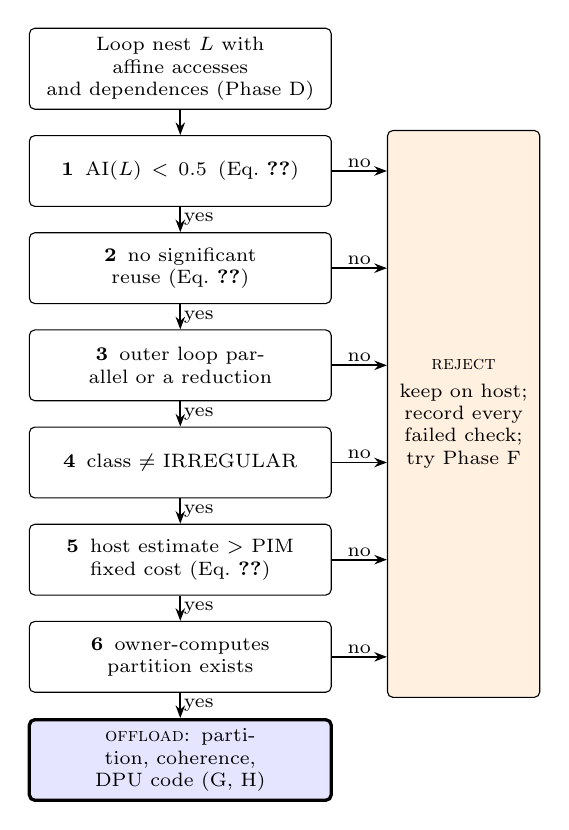
\begin{tikzpicture}[node distance=3.2mm]
\node[blk=36mm] (n0) {Loop nest $L$ with affine accesses\\and dependences (Phase D)};
\node[blk=36mm, below=of n0] (c1) {\textbf{1}\enspace $\mathrm{AI}(L) < 0.5$\enspace (Eq.~\ref{eq:ai})};
\node[blk=36mm, below=of c1] (c2) {\textbf{2}\enspace no significant reuse (Eq.~\ref{eq:reuse})};
\node[blk=36mm, below=of c2] (c3) {\textbf{3}\enspace outer loop parallel or a reduction};
\node[blk=36mm, below=of c3] (c4) {\textbf{4}\enspace class $\ne$ IRREGULAR};
\node[blk=36mm, below=of c4] (c5) {\textbf{5}\enspace host estimate $>$ PIM fixed cost (Eq.~\ref{eq:size})};
\node[blk=36mm, below=of c5] (c6) {\textbf{6}\enspace owner-computes partition exists};
\node[blk=36mm, below=of c6, fill=blue!10, very thick] (ok) {\textsc{offload}: partition, coherence,\\DPU code (G, H)};
\node[blk=17mm, minimum height=72mm, fill=orange!12, anchor=west] (rej) at ($(c3.east)!0.5!(c4.east) + (7mm,0)$) {\textsc{reject}\\[2pt]keep on host;\\record every\\failed check;\\try Phase F};
\draw[arr] (n0) -- (c1);
\draw[arr] (c1) -- node[lbl, right] {yes} (c2);
\draw[arr] (c2) -- node[lbl, right] {yes} (c3);
\draw[arr] (c3) -- node[lbl, right] {yes} (c4);
\draw[arr] (c4) -- node[lbl, right] {yes} (c5);
\draw[arr] (c5) -- node[lbl, right] {yes} (c6);
\draw[arr] (c6) -- node[lbl, right] {yes} (ok);
\foreach \c in {c1,c2,c3,c4,c5,c6} \draw[arr] (\c.east) -- node[lbl, above] {no} (\c.east -| rej.west);
\end{tikzpicture}
\caption{Offload decision of Phase E (Algorithm~\ref{alg:decide}). All checks are evaluated so that the explanation lists every reason; a nest is offloaded only if all six hold.}
\label{fig:decision}
\end{figure}

\subsubsection{Enabling Transformations}
When a nest is rejected, three classical transformations are tried, each checked for legality on the dependence graph, and the resulting nests are decided again by Algorithm~\ref{alg:decide}. Fig.~\ref{fig:transform} shows one example of each.

\emph{Loop fission} follows Allen and Kennedy: the statements of the loop form a graph whose edges are the dependences between them, Tarjan's algorithm finds its strongly connected components, and the components are emitted in topological order, one loop each. In \texttt{mixed\_loop}, a parallel statement \texttt{B[i]=A[i]*2} shares a loop with the recurrence \texttt{C[i]=C[i-1]+D[i]}; fission separates them, and the first loop is offloaded while the second stays on the host.

\emph{Loop interchange} permutes the loops of a nest; a permutation is legal when every direction vector remains lexicographically non-negative. In \texttt{colmajor}, the inner loop walks down a column with a 512-byte stride and the outer loop does not follow the partitioned dimension; swapping the loops makes the inner access contiguous and the outer loop partitionable, and the counted memory traffic falls from 2,097,152 to 131,072 bytes.

\emph{Loop fusion} merges adjacent loops with the same bounds when no dependence would point backwards in the fused loop. In \texttt{fusion\_chain}, the intermediate array \texttt{T} is produced by one loop and consumed by the next; after fusion it never leaves the DPUs, which saves one launch (80,000 cycles) and 131,072 bytes of DMA.

\begin{figure}[!t]
\centering
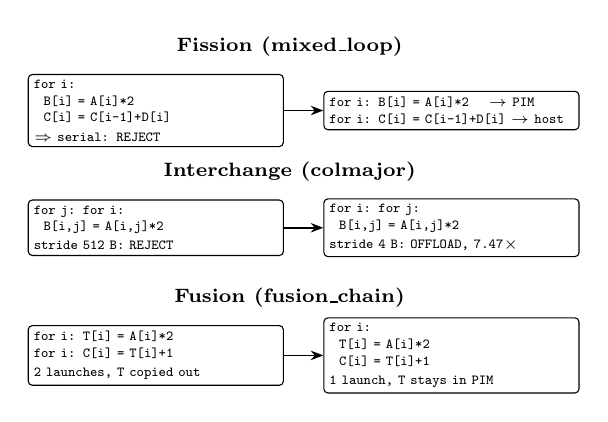
\begin{tikzpicture}[node distance=2.5mm and 5mm,
  code/.style={draw, rounded corners=1.5pt, align=left, font=\ttfamily\tiny, text width=31mm, inner sep=2pt, fill=white},
  ttl/.style={font=\scriptsize\bfseries}]
\node[ttl] (t1) {Fission (mixed\_loop)};
\node[code, below=1mm of t1, xshift=-17mm] (a1) {for i:\\\ \ B[i] = A[i]*2\\\ \ C[i] = C[i-1]+D[i]\\[1pt]$\Rightarrow$ serial: REJECT};
\node[code, right=of a1] (b1) {for i: B[i] = A[i]*2\ \ \ \ $\rightarrow$ PIM\\for i: C[i] = C[i-1]+D[i]\ $\rightarrow$ host};
\draw[arr] (a1) -- (b1);
\node[ttl, below=11mm of t1] (t2) {Interchange (colmajor)};
\node[code, below=1mm of t2, xshift=-17mm] (a2) {for j: for i:\\\ \ B[i,j] = A[i,j]*2\\[1pt]stride 512 B: REJECT};
\node[code, right=of a2] (b2) {for i: for j:\\\ \ B[i,j] = A[i,j]*2\\[1pt]stride 4 B: OFFLOAD, 7.47$\times$};
\draw[arr] (a2) -- (b2);
\node[ttl, below=11mm of t2] (t3) {Fusion (fusion\_chain)};
\node[code, below=1mm of t3, xshift=-17mm] (a3) {for i: T[i] = A[i]*2\\for i: C[i] = T[i]+1\\[1pt]2 launches, T copied out};
\node[code, right=of a3] (b3) {for i:\\\ \ T[i] = A[i]*2\\\ \ C[i] = T[i]+1\\[1pt]1 launch, T stays in PIM};
\draw[arr] (a3) -- (b3);
\end{tikzpicture}
\caption{The three enabling transformations on the benchmarks where they apply. Each is checked for legality on the dependence graph, and the result is decided again.}
\label{fig:transform}
\end{figure}

\subsubsection{Partitioning and Coherence}
\label{sec:partcoh}
An offloaded nest is divided among the DPUs by the owner-computes rule: each DPU owns a contiguous block of rows of every array (dimension 0) and executes exactly the iterations that write rows it owns; with 16,384 iterations and 64 DPUs each DPU receives 256. Every read is then classified as local (same access function), halo (a constant offset $\delta$ on the partitioned dimension, which needs $|\delta|$ neighbouring rows), broadcast (a small array every DPU needs), private (a reduction accumulator, merged afterwards) or impossible (a write whose row does not follow the partitioned loop). The last case is the canonical failure of transpose: every DPU would write a column of \texttt{B[j,i]} spread over all other DPUs' rows, an all-to-all exchange that the hardware cannot perform. Block, cyclic and block-cyclic distributions are scored by halo bytes plus a fixed cost per separate transfer run, and the cheapest is chosen; for stencil1d the scores are 77,304 for block, 1,236,992 for block-cyclic and 19,789,456 for cyclic.

The host's cache and the DPUs' copies of an array can disagree, so NEMO-C inserts \texttt{flush(X)} before a kernel reads an array the host has written and \texttt{invalidate(X)} before the host reads an array a kernel has written. The placement is a forward dataflow analysis over the host CFG, whose facts are pairs of sets of arrays: $H$ (written by the host, not yet flushed) and $P$ (written on the DPUs, not yet invalidated in the host cache). The meet over predecessors is set union and the transfer function of a block $b$ is applied statement by statement:
\begin{equation}
\begin{aligned}
\mathrm{IN}(b) &= \textstyle\bigcup_{p\in\mathrm{pred}(b)} \mathrm{OUT}(p),\\
\mathrm{OUT}(b) &= \big(\mathrm{IN}(b) \setminus \mathrm{KILL}(b)\big) \cup \mathrm{GEN}(b),
\end{aligned}
\label{eq:dataflow}
\end{equation}
where a host store of $X$ generates $X$ in $H$, a kernel that reads $X\in H$ requires a flush and kills $X$ from $H$, a kernel that writes $X$ generates $X$ in $P$, and a host load of $X\in P$ requires an invalidate and kills $X$ from $P$. Algorithm~\ref{alg:coherence} iterates (\ref{eq:dataflow}) to a fixed point and then inserts the operations. Union is the safe meet: if an array is stale on any path into a block, the block must treat it as stale. Fig.~\ref{fig:coherence} shows the effect on a program in which the host reads the kernel's output inside one branch of an \texttt{if} and again after it. The path that skips the branch still carries $C\in P$, so the read after the merge needs its own invalidate. The analysis reaches its fixed point in three rounds, because the loop's back edge carries $H=\{A\}$ to the loop header in the second round.

\begin{algorithm}[!t]
\caption{Placement of flush and invalidate operations}
\label{alg:coherence}
\begin{algorithmic}[1]
\REQUIRE host CFG $G=(V,E)$; for each kernel call, the arrays it reads and writes
\ENSURE IR with \texttt{flush} and \texttt{invalidate} inserted
\FORALL{$b \in V$} \STATE $\mathrm{OUT}(b) \leftarrow (\emptyset,\emptyset)$ \ENDFOR
\REPEAT
  \STATE $changed \leftarrow$ \FALSE
  \FORALL{$b \in V$ in reverse post-order}
    \STATE $(H,P) \leftarrow \bigcup_{p\in\mathrm{pred}(b)} \mathrm{OUT}(p)$
    \FORALL{statement $s$ in $b$}
      \IF{$s$ stores array $X$} \STATE $H \leftarrow H\cup\{X\}$ \ENDIF
      \IF{$s$ calls a kernel} \STATE $H \leftarrow H \setminus \mathrm{reads}(s)$;\ $P \leftarrow P \cup \mathrm{writes}(s)$ \ENDIF
      \IF{$s$ loads array $X \in P$} \STATE $P \leftarrow P \setminus\{X\}$ \ENDIF
    \ENDFOR
    \IF{$(H,P) \ne \mathrm{OUT}(b)$} \STATE $\mathrm{OUT}(b)\leftarrow(H,P)$;\ $changed \leftarrow$ \TRUE \ENDIF
  \ENDFOR
\UNTIL{\NOT $changed$}
\STATE replay each block from its fixed-point IN set; insert \texttt{flush(X)} where a call reads $X\in H$ and \texttt{invalidate(X)} where a load reads $X\in P$
\end{algorithmic}
\end{algorithm}

\begin{figure}[!t]
\centering
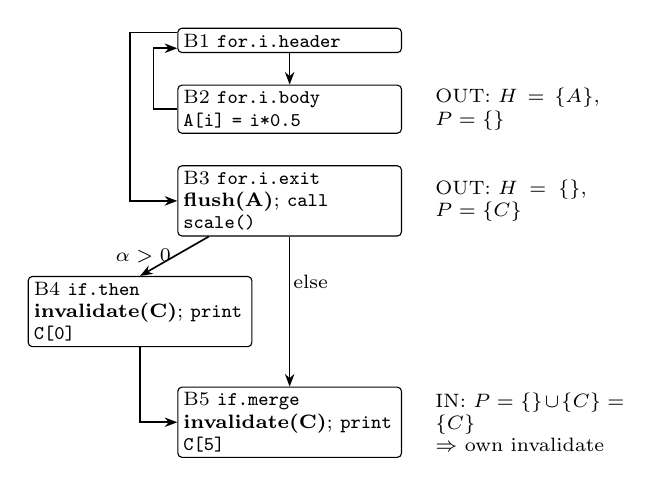
\begin{tikzpicture}[node distance=4mm,
  cb/.style={draw, rounded corners=1.5pt, align=left, font=\scriptsize, text width=27mm, inner sep=2pt, fill=white},
  st/.style={font=\scriptsize, align=left, text width=24mm}]
\node[cb] (b1) {B1 \texttt{for.i.header}};
\node[cb, below=of b1] (b2) {B2 \texttt{for.i.body}\\\texttt{A[i] = i*0.5}};
\node[cb, below=of b2] (b3) {B3 \texttt{for.i.exit}\\\textbf{flush(A)}; \texttt{call scale()}};
\node[cb, below=5mm of b3, xshift=-19mm] (b4) {B4 \texttt{if.then}\\\textbf{invalidate(C)}; \texttt{print C[0]}};
\node[cb, below=5mm of b4, xshift=19mm] (b5) {B5 \texttt{if.merge}\\\textbf{invalidate(C)}; \texttt{print C[5]}};
\node[st, right=3mm of b2] {OUT: $H=\{A\}$, $P=\{\}$};
\node[st, right=3mm of b3] {OUT: $H=\{\}$, $P=\{C\}$};
\node[st, right=3mm of b5] {IN: $P=\{\}\cup\{C\}=\{C\}$\\$\Rightarrow$ own invalidate};
\draw[arr] (b1) -- (b2);
\draw[arr] (b2.west) -- ++(-3mm,0) |- ([yshift=-1mm]b1.west);
\draw[arr] ([yshift=1mm]b1.west) -- ++(-6mm,0) |- (b3.west);
\draw[arr] ([xshift=4mm]b3.south west) -- node[lbl, left] {$\alpha>0$} (b4.north);
\draw[arr] (b4.south) |- (b5.west);
\draw[arr] (b3.south) -- node[lbl, right, pos=0.3] {else} (b5.north);
\end{tikzpicture}
\caption{Coherence analysis on \texttt{coherence\_demo}. At the merge block B5 the union of $P=\{\}$ (through B4) and $P=\{C\}$ (skipping B4) is $\{C\}$, so the second read of \texttt{C} needs its own invalidate.}
\label{fig:coherence}
\end{figure}

\subsubsection{Code Generation and Register Allocation}
For each offloaded nest the back end selects instructions of a small PIM instruction set (\texttt{LD}, \texttt{ST}, \texttt{ADD}, \texttt{SUB}, \texttt{MUL}, \texttt{DIV}, \texttt{MOVI}, \texttt{DMA\_IN}, \texttt{DMA\_OUT}, \texttt{LOOP}, \texttt{ENDLOOP} and \texttt{HALO\_EXCHANGE}, extended with comparisons, \texttt{MOV}, \texttt{MIN}, \texttt{ARG}/\texttt{RET} and floating-point variants so that conditionals and reductions can be expressed). Because a DPU computes only from its 64\,KB scratchpad, the generated code processes its slice in tiles of $T$ iterations, with
\begin{equation}
T = \left\lfloor \frac{W - W_{\mathrm{spill}} - W_{\mathrm{res}} - W_{\mathrm{halo}}}{b_{\mathrm{iter}}} \right\rfloor,
\label{eq:tile}
\end{equation}
where $W=65{,}536$ bytes, $W_{\mathrm{spill}}$ is the spill area, $W_{\mathrm{res}}$ holds broadcast arrays, $W_{\mathrm{halo}}$ the halo rows, and $b_{\mathrm{iter}}$ the bytes one iteration moves; for stencil1d, $T=\lfloor(65{,}536-512-0-8)/8\rfloor=8{,}127$. The arithmetic is written as a comment at the top of every generated file.

Registers are allocated by Chaitin--Briggs graph colouring with $K=24$ physical registers (Algorithm~\ref{alg:regalloc}, Fig.~\ref{fig:regalloc}). Liveness is computed by a backward dataflow analysis over the DPU program, $\mathrm{in}(n)=\mathrm{use}(n)\cup(\mathrm{out}(n)\setminus\mathrm{def}(n))$, and two virtual registers interfere when one is defined while the other is live. Copy-related registers are merged first by the Briggs conservative test, which allows a merge only if the merged node has fewer than $K$ neighbours of degree at least $K$, so coalescing can never make a colourable graph uncolourable. Nodes of degree below $K$ are then removed onto a stack; when none remains, the node with the lowest spill priority
\begin{equation}
\mathrm{prio}(v) = \frac{\sum_{x\in \mathrm{defs}(v)\cup\mathrm{uses}(v)} 10^{\,\mathrm{depth}(x)}}{\deg(v)}
\label{eq:spill}
\end{equation}
is pushed optimistically. Popping the stack assigns each node the lowest colour not used by its neighbours; a node that finds none is spilled to the scratchpad with a load before each use and a store after each definition, and the whole process repeats. Finally, the host side is generated as C code that flushes, splits the iterations among the 64 DPUs, transfers each DPU's rows with their halo, launches and waits for the DPUs, copies the results back and merges reductions.

\begin{algorithm}[!t]
\caption{Chaitin--Briggs register allocation}
\label{alg:regalloc}
\begin{algorithmic}[1]
\REQUIRE DPU program over virtual registers; $K=24$
\ENSURE colouring $\kappa: V\rightarrow\{1,\dots,K\}$ with $\kappa(u)\ne\kappa(v)$ for every interference edge
\REPEAT
  \STATE compute liveness; build interference graph $G=(V,E)$
  \STATE coalesce copy pairs that pass the Briggs test
  \STATE $S \leftarrow$ empty stack
  \WHILE{$V \ne \emptyset$}
    \IF{some $v$ has $\deg(v) < K$} \STATE push $v$ on $S$; remove $v$ \ELSE \STATE push $\arg\min_v \mathrm{prio}(v)$ by (\ref{eq:spill}); remove it \ENDIF
  \ENDWHILE
  \STATE $spilled \leftarrow \emptyset$
  \WHILE{$S$ not empty}
    \STATE pop $v$; give it the lowest colour unused by coloured neighbours
    \IF{no colour is free} \STATE $spilled \leftarrow spilled \cup \{v\}$ \ENDIF
  \ENDWHILE
  \STATE insert spill loads and stores for every $v \in spilled$
\UNTIL{$spilled = \emptyset$}
\RETURN $\kappa$
\end{algorithmic}
\end{algorithm}

\begin{figure}[!t]
\centering
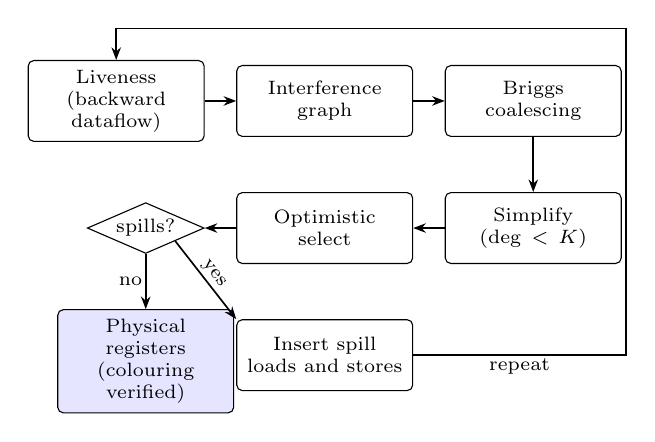
\begin{tikzpicture}[node distance=4mm and 4mm]
\node[blk=20mm] (r1) {Liveness\\(backward dataflow)};
\node[blk=20mm, right=of r1] (r2) {Interference\\graph};
\node[blk=20mm, right=of r2] (r3) {Briggs\\coalescing};
\node[blk=20mm, below=7mm of r3] (r4) {Simplify\\($\deg < K$)};
\node[blk=20mm, left=of r4] (r5) {Optimistic\\select};
\node[dec, left=of r5] (r6) {spills?};
\node[blk=20mm, below=7mm of r5] (r7) {Insert spill\\loads and stores};
\node[blk=20mm, below=7mm of r6, fill=blue!10] (r8) {Physical registers\\(colouring verified)};
\draw[arr] (r1) -- (r2);
\draw[arr] (r2) -- (r3);
\draw[arr] (r3) -- (r4);
\draw[arr] (r4) -- (r5);
\draw[arr] (r5) -- (r6);
\draw[arr] (r6) -- node[lbl, left] {no} (r8);
\draw[arr] (r6.south east) -- node[lbl, above, sloped] {yes} (r7.north west);
\draw[arr] (r7.east) -- node[lbl, below] {repeat} ++(27mm,0) |- ([yshift=4mm]r1.north) -- (r1.north);
\end{tikzpicture}
\caption{Chaitin--Briggs register allocation (Algorithm~\ref{alg:regalloc}). Spilling changes the program, so the process repeats until every virtual register has a physical register.}
\label{fig:regalloc}
\end{figure}

\subsubsection{Simulation and Validation}
Because no PIM hardware was available, NEMO-C includes a simulator that both executes and costs the program. The host model is a 32\,KB, 8-way set-associative LRU cache with 64-byte lines; a hit costs 4 cycles, a miss 100, and each line fill or write-back puts 64 bytes on the bus. For an offloaded nest the simulated time is
\begin{equation}
\begin{aligned}
T_{\mathrm{pim}} ={}& c_{\mathrm{launch}} + \underbrace{c_{\mathrm{dma}}B + c_{\mathrm{run}}N_{\mathrm{run}} + c_{\mathrm{set}}N_{\mathrm{set}}}_{\text{DMA in and out}}\\
&+ \max_{d} T_{\mathrm{dpu}}(d) + T_{\mathrm{merge}},
\end{aligned}
\label{eq:pimtime}
\end{equation}
where $N_{\mathrm{run}}$ counts separate contiguous transfer segments, $N_{\mathrm{set}}$ the per-array transfer sets, and $T_{\mathrm{dpu}}(d)$ the cycles of DPU $d$: 2 per ALU operation, 16 per multiply, 32 per divide, and 10 per scratchpad access divided by the overlap of $\min(16,11)$ tasklets and multiplied by a bank-conflict factor for strides that are multiples of the bank count. Each DPU sees a private image of the arrays in which only the rows the partition assigned to it are present, so a wrong partition or halo is detected as an access error, and two DPUs writing the same element are reported as a race. The results of every configuration are compared bit for bit with the host-only run, the unoptimised IR is run once more to check the optimiser, and the generated, register-allocated DPU programs are executed by an interpreter (\texttt{dpu\_interp.cpp}) and must agree as well. The speedup of a configuration is
\begin{equation}
S_{\mathrm{cfg}} = \frac{T_{\textsc{host\_only}}}{T_{\mathrm{cfg}}}.
\label{eq:speedup}
\end{equation}

% =============================================================================
\section{Implementation and Result Analysis}
\label{sec:results}
% =============================================================================

\subsection{Tools, Configuration and Setup}
NEMO-C is written in C++17 using only the standard library. The scanner is generated by Flex 2.6.4 and the LALR(1) parser by GNU Bison 3.8.2 \cite{bison2021manual}; the compiler, the test programs and the generated host code are built with GCC (g++ 15.2) \cite{gcc2024manual} through a plain GNU Make 4.4.1 build. The experiments ran under Ubuntu 26.04 LTS in WSL2 on a laptop with a 13th-generation Intel Core i7-1360P processor (16 hardware threads) and 7\,GB of memory available to the Linux environment. Plots are drawn by a separate Python script with Matplotlib \cite{matplotlib2024}, kept outside the compiler, and a browser workbench served by a Python standard-library server drives the same compiler binary for demonstration.

The project is built with \texttt{make}; \texttt{./nemoc prog.nmc -{}-decisions} prints one verdict per nest, \texttt{-{}-explain <kernel>} prints the full decision trace, \texttt{-{}-codegen} writes the DPU assembly and host C, \texttt{-{}-dump regalloc -{}-regs K} prints the allocation for a register budget $K$, and \texttt{-{}-simulate} runs the three configurations. The command \texttt{make test} builds and runs the eight test programs, and \texttt{make run-all} simulates all benchmarks and writes \texttt{results/results.csv}, from which every number in this section is taken. Fig.~\ref{fig:screenshot} shows the workbench executing \texttt{-{}-explain} on matrix multiplication.

\begin{figure*}[!t]
\centering
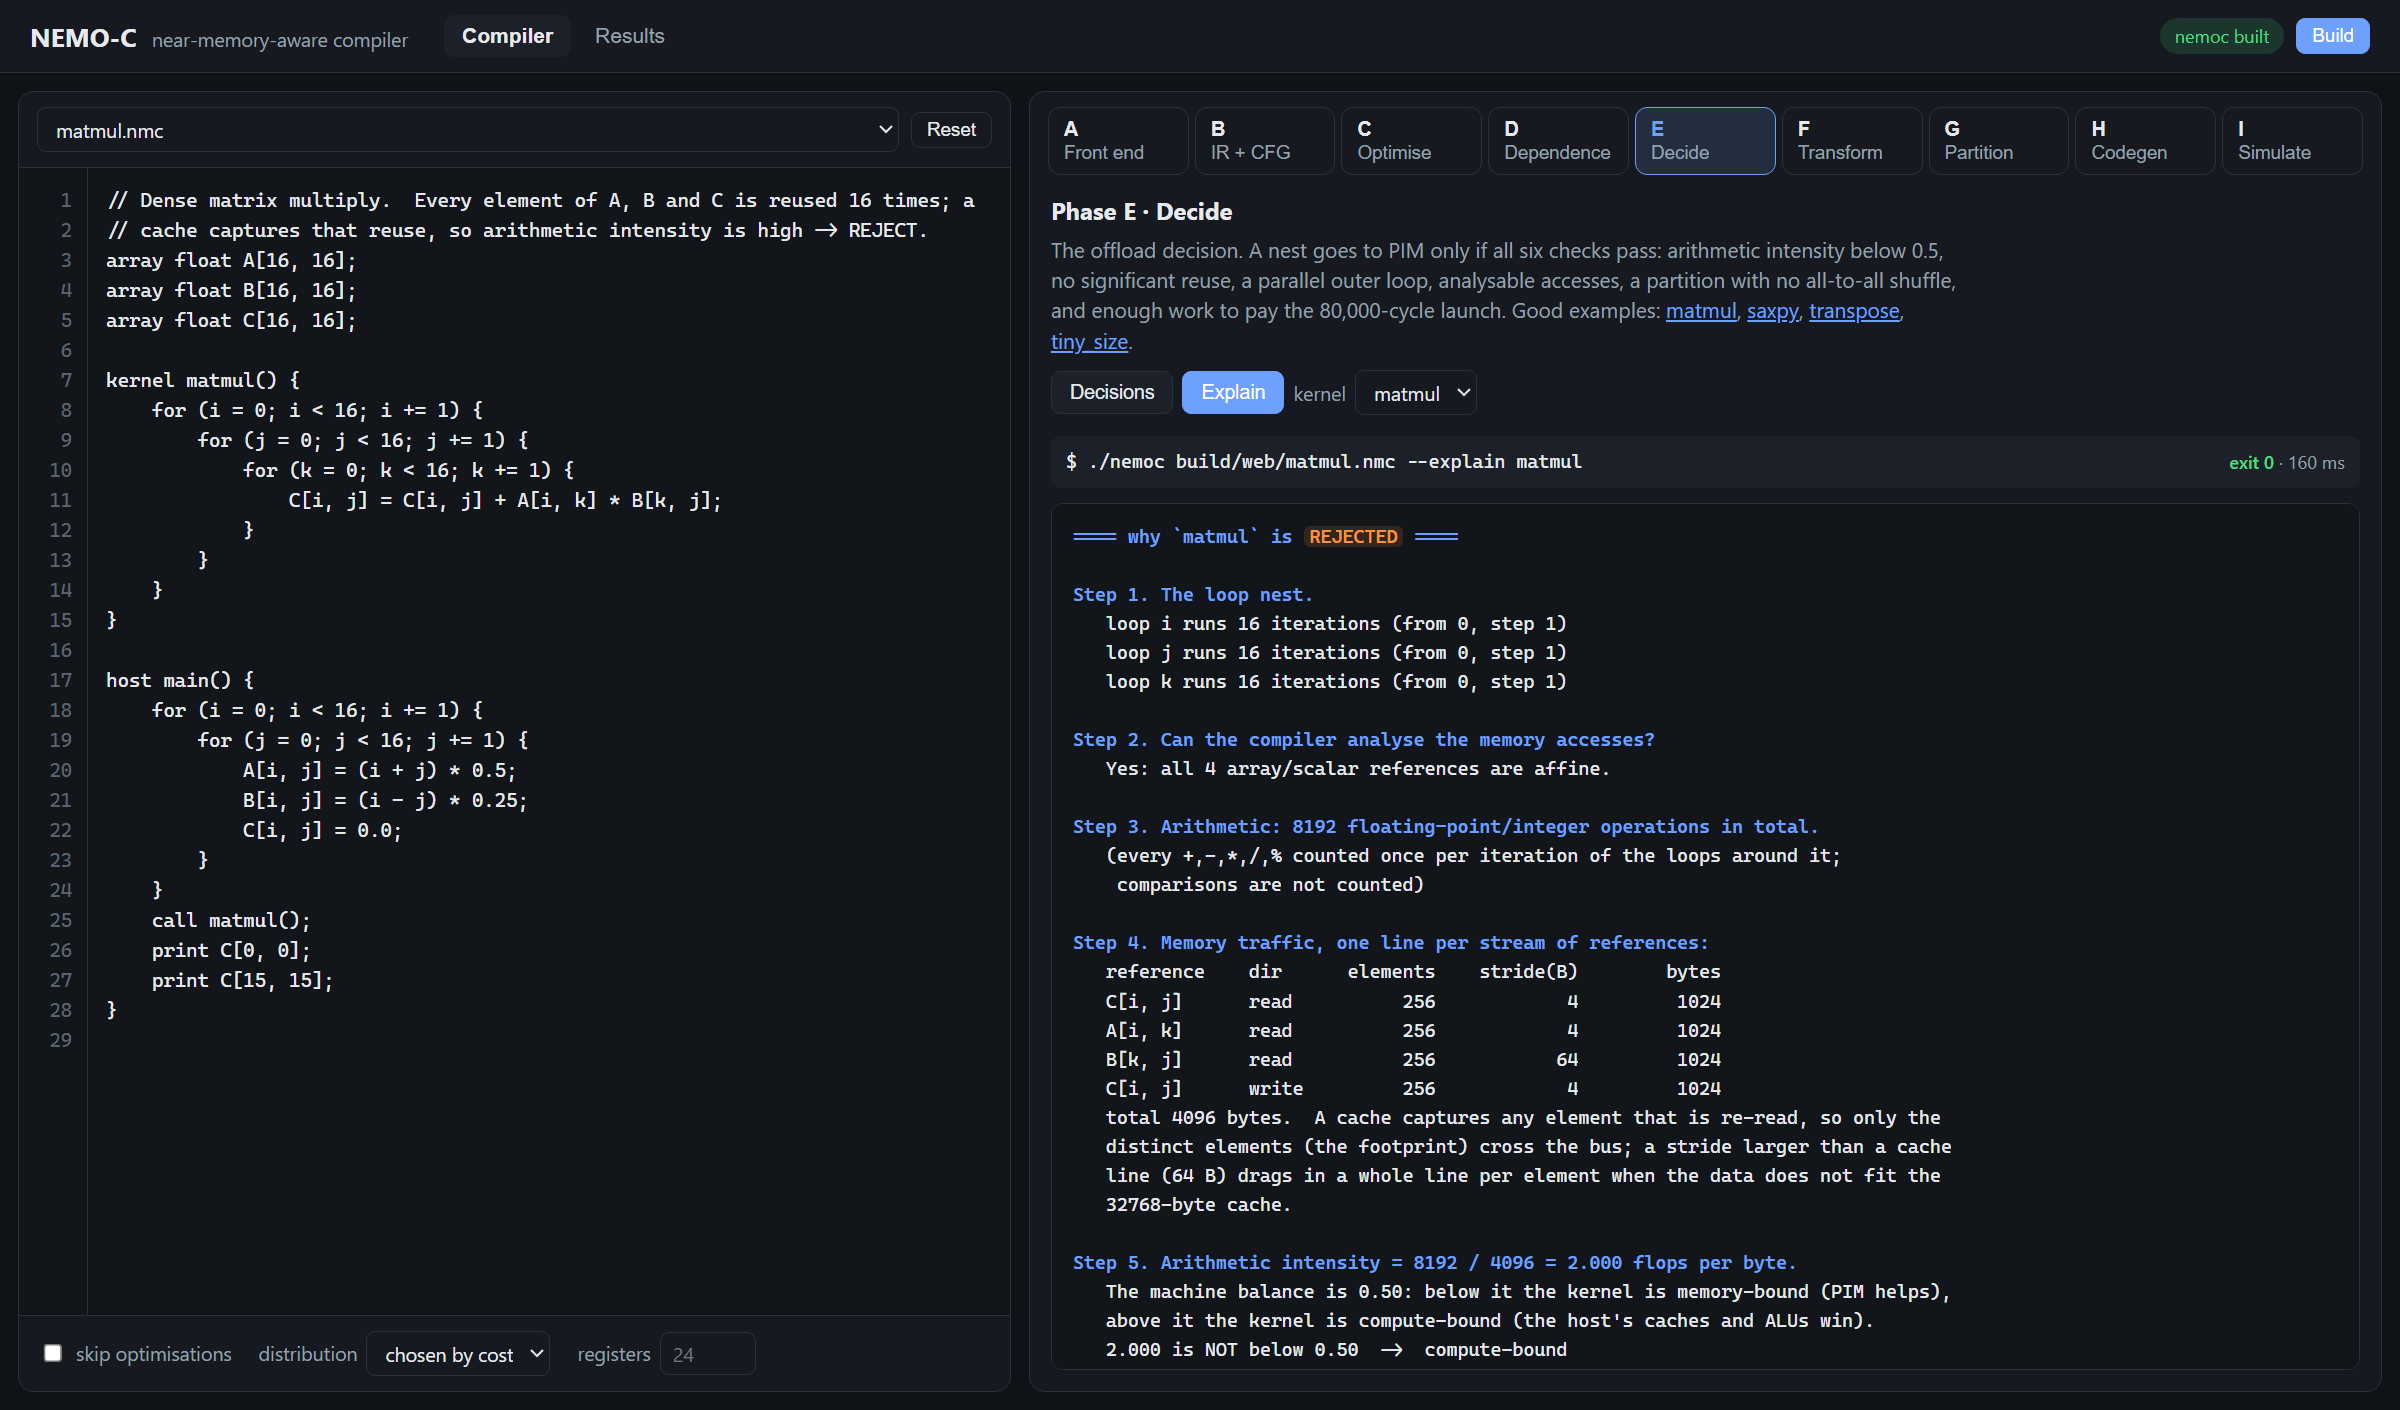
\includegraphics[width=0.92\textwidth]{figures/workbench.png}
\caption{The NEMO-C workbench running \texttt{./nemoc matmul.nmc -{}-explain matmul}. The left pane holds the program; the right pane shows phases A--I and the compiler's decision trace, which reports $\mathrm{AI}=8192/4096=2.0$ and rejects the nest.}
\label{fig:screenshot}
\end{figure*}

\subsection{Parameter Setup}
Table~\ref{tab:params} lists the parameters of the machine model. The first group is given by the course specification of the target; the second was added to complete the model, and each value is justified in the source file \texttt{config.h}. All benchmarks use 16,384 one-dimensional elements or $128\times128$ matrices, except matrix multiplication ($16\times16$) and the histogram (256 bins over 16,384 inputs).

\begin{table}[!t]
\caption{Parameters of the machine model (\texttt{config.h}).}
\label{tab:params}
\setlength{\tabcolsep}{3pt}
\renewcommand{\arraystretch}{1.1}
\centering
\begin{tabular}{|p{4.6cm}|p{2.9cm}|}
\hline
\textbf{Parameter} & \textbf{Value} \\ \hline
DPUs $P$; tasklets per DPU & 64; 16 \\ \hline
Scratchpad (WRAM) per DPU & 65,536 bytes \\ \hline
DPU registers $K$ & 24 \\ \hline
Host cache hit / miss & 4 / 100 cycles \\ \hline
Host ALU operation & 1 cycle \\ \hline
DPU ALU / multiply / divide & 2 / 16 / 32 cycles \\ \hline
DPU scratchpad access & 10 cycles \\ \hline
DMA per byte & 0.5 cycle \\ \hline
Machine balance & 0.5 flop/byte \\ \hline
Cache line & 64 bytes \\ \hline
Energy: DRAM line / PIM access / ALU & 640 / 60 / 1 pJ \\ \hline
\multicolumn{2}{|l|}{\emph{Added to complete the model}} \\ \hline
Launch and synchronisation overhead & 80,000 cycles \\ \hline
DMA setup per transfer set / per run & 2,000 / 300 cycles \\ \hline
Host cache size and associativity & 32 KB, 8-way LRU \\ \hline
Tasklets that saturate the pipeline & 11 \\ \hline
Memory banks per DPU & 8 \\ \hline
Reuse significance threshold $\rho$ & 0.10 \\ \hline
\end{tabular}
\end{table}

\subsection{Benchmarks and Decisions}
Table~\ref{tab:bench} lists the fifteen benchmarks, their class and arithmetic intensity as computed by Phase E, and the verdict. They were chosen to cover every case the decision must handle: streaming element-wise kernels, reductions, stencils, a matrix--vector product with negligible reuse, three kernels that need one of the enabling transformations, and three that must be rejected for three different reasons.

\begin{table}[!t]
\caption{Benchmarks and NEMO-C verdicts (AI in flop/byte).}
\label{tab:bench}
\setlength{\tabcolsep}{2.5pt}
\renewcommand{\arraystretch}{1.08}
\centering
\begin{tabular}{|p{1.45cm}|p{1.9cm}|p{0.65cm}|p{3.5cm}|}
\hline
\textbf{Benchmark} & \textbf{Class} & \textbf{AI} & \textbf{Verdict and reason} \\ \hline
vecadd & elementwise & 0.08 & OFFLOAD \\ \hline
saxpy & elementwise & 0.17 & OFFLOAD \\ \hline
dotprod & reduction & 0.25 & OFFLOAD (integer sum) \\ \hline
maxreduce & reduction & 0.00 & OFFLOAD (conditional max) \\ \hline
histogram & reduction & 0.24 & OFFLOAD (private histograms) \\ \hline
gemv & elementwise & 0.49 & OFFLOAD (reuse 1\% of bytes) \\ \hline
stencil1d & stencil & 0.37 & OFFLOAD (halo 1 row) \\ \hline
stencil2d & stencil & 0.49 & OFFLOAD (halo) \\ \hline
filter & elementwise & 0.00 & OFFLOAD (data-dependent if) \\ \hline
fusion\_chain & elementwise & 0.12 & OFFLOAD after fusion \\ \hline
mixed\_loop & mixed & 0.12 & 1 of 2 loops after fission \\ \hline
colmajor & elementwise & 0.12 & OFFLOAD after interchange \\ \hline
matmul & compute-bound & 2.00 & REJECT: AI, reuse, size \\ \hline
transpose & elementwise & 0.00 & REJECT: all-to-all partition \\ \hline
indirect & irregular & n/a & REJECT: non-affine \texttt{A[B[i]]} \\ \hline
\end{tabular}
\end{table}

Three configurations are simulated for each benchmark. HOST\_ONLY runs everything on the CPU. NAIVE\_OFFLOAD offloads every parallel loop without consulting the cost model and without the enabling transformations, which is what a programmer obtains by porting every parallel kernel to the DPUs. NEMO-C applies Algorithm~\ref{alg:decide} and the transformations. We report six performance metrics: execution time (as speedup), memory-bus traffic, energy, decision correctness, register pressure and compile time, together with the correctness checks.

\subsection{Metric 1: Execution Time}
Fig.~\ref{fig:speedup} shows the speedup of both offloading configurations over HOST\_ONLY. NEMO-C is never slower than the host. For the nine benchmarks that offload as written, NEMO-C and NAIVE\_OFFLOAD make the same choice and gain between 1.01$\times$ (histogram, where merging 64 private histograms on the host absorbs most of the benefit) and 1.68$\times$ (stencil2d, where the host performs several reads per element). The transformations give the largest gains: 7.47$\times$ for colmajor after interchange, against 0.71$\times$ when the column-order loop is offloaded unchanged; 2.08$\times$ for fusion\_chain after fusion, against 1.46$\times$; and 1.12$\times$ for mixed\_loop after fission, where blind offloading cannot offload anything. On the three rejected benchmarks NAIVE\_OFFLOAD runs at 0.63$\times$ (matmul), 0.70$\times$ (transpose) and 0.43$\times$ (indirect), while NEMO-C matches the host exactly. Over all fifteen benchmarks the total simulated time is 15.48\,M cycles for HOST\_ONLY, 17.49\,M for NAIVE\_OFFLOAD (0.89$\times$) and 10.20\,M for NEMO-C (1.52$\times$). The justification is the cost model itself: the rejected nests are precisely those in which launch, DMA and lost cache reuse cost more than near-memory execution saves.

\begin{figure}[!t]
\centering
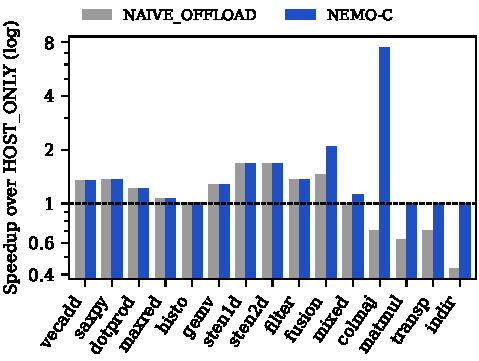
\includegraphics[width=\columnwidth]{figures/fig_speedup.pdf}
\caption{Metric 1: speedup over HOST\_ONLY (log scale; Eq.~\ref{eq:speedup}). NEMO-C never falls below 1.0; blind offloading loses on colmajor, matmul, transpose and indirect.}
\label{fig:speedup}
\end{figure}

\subsection{Metric 2: Memory-Bus Traffic}
Fig.~\ref{fig:traffic} shows the bytes that cross the memory bus, normalised to HOST\_ONLY. For streaming kernels offloading moves roughly the same bytes as the host (0.84--1.33$\times$), because every operand is copied in and every result copied out once. The differences appear where locality differs. NEMO-C moves 0.08$\times$ the host's bytes on colmajor, because the host drags a 64-byte line per element along a column while the transformed DPU code moves contiguous rows, and 0.52$\times$ on fusion\_chain, because the intermediate array never leaves PIM. Blind offloading of matmul moves 8.4$\times$ the host's bytes, because the whole of \texttt{B} is broadcast to every DPU while the host serves it from its cache, and of indirect 6.4$\times$, because every DPU needs all of \texttt{A}. Transpose shows that traffic alone is not the criterion: blind offloading moves only 0.12$\times$ the bytes, yet runs 0.70$\times$ slower, because its output is split into 8,192 separate transfer segments. In total NEMO-C moves 6.95\,MB against 10.35\,MB for the host and 13.15\,MB for blind offloading.

\begin{figure}[!t]
\centering
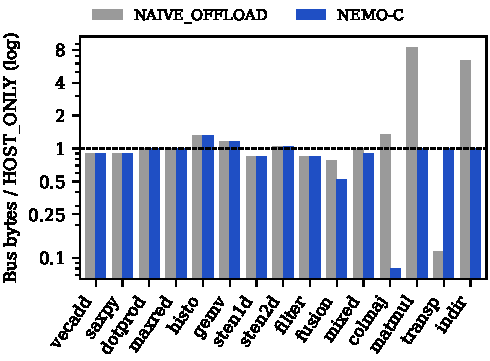
\includegraphics[width=\columnwidth]{figures/fig_traffic.pdf}
\caption{Metric 2: memory-bus bytes normalised to HOST\_ONLY (log scale).}
\label{fig:traffic}
\end{figure}

\subsection{Metric 3: Energy}
Fig.~\ref{fig:energy} shows energy normalised to HOST\_ONLY. Over the whole set NEMO-C uses 73.3\,$\mu$J against 105.1\,$\mu$J for the host (0.70$\times$) and 143.4\,$\mu$J for blind offloading (1.36$\times$). Most of the saving comes from colmajor (0.09$\times$) and fusion\_chain (0.56$\times$), and the rejections avoid the 6.9$\times$ energy of blind offloading on matmul and indirect. Two results are less favourable and we report them as measured. Several offloaded streaming kernels use slightly more energy than the host (up to 1.39$\times$ for histogram and 1.23$\times$ for gemv), because each DMA burst costs a DRAM access plus a bank access. And transpose under blind offloading uses less energy than the host (0.13$\times$) although it is slower. NEMO-C's rule optimises time, not energy, which is a limitation discussed below.

\begin{figure}[!t]
\centering
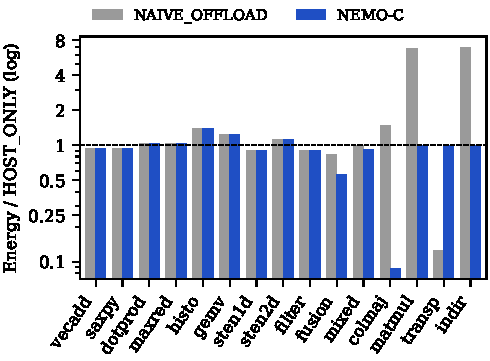
\includegraphics[width=\columnwidth]{figures/fig_energy.pdf}
\caption{Metric 3: energy normalised to HOST\_ONLY (log scale).}
\label{fig:energy}
\end{figure}

\subsection{Metric 4: Decision Correctness and Comparison with Related Work}
We compare NEMO-C with three related works by implementing their offload policies in the same simulator, since their tool chains do not accept our source language. The \emph{offload-all} policy corresponds to the hand-ported workloads of PrIM \cite{gomezluna2022prim} and to programmer-directed frameworks such as SimplePIM \cite{chen2023simplepim}, in which every kernel the programmer marks runs on PIM; it is our NAIVE\_OFFLOAD configuration. The \emph{AI-only} policy represents a single-metric roofline rule that offloads whenever $\mathrm{AI}<0.5$, ignoring reuse, partitionability and size. Devic \emph{et al.} \cite{devic2022topim} make selective decisions for bank-level RISC-V cores; their framework is not reproduced quantitatively here, and Table~\ref{tab:compare} compares it qualitatively. A decision is counted as correct when its time is no worse than the better of HOST\_ONLY and NAIVE\_OFFLOAD for that benchmark.

Fig.~\ref{fig:policy} and Table~\ref{tab:compare} give the outcome. Offload-all reaches a geometric-mean speedup of 1.06$\times$ with four slowdowns (worst 0.43$\times$) and 11 of 15 correct decisions; AI-only reaches 1.09$\times$ with three slowdowns and 12 correct decisions, because it rejects matmul but cannot see the all-to-all partition of transpose, the irregularity of indirect or the stride of colmajor. NEMO-C reaches 1.42$\times$ with no slowdown and 15 of 15 correct decisions, and on three benchmarks it exceeds both simple choices because the transformations create options that neither policy has.

\begin{figure}[!t]
\centering
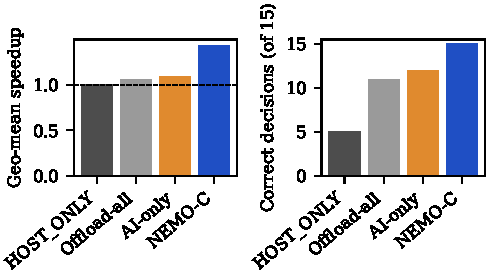
\includegraphics[width=\columnwidth]{figures/fig_policy.pdf}
\caption{Metric 4: geometric-mean speedup and number of decisions that are no worse than the better of HOST\_ONLY and NAIVE\_OFFLOAD, for four offload policies over the 15 benchmarks.}
\label{fig:policy}
\end{figure}

\begin{table}[!t]
\caption{Comparison with related work. Quantitative rows use the same simulator and 15 benchmarks.}
\label{tab:compare}
\setlength{\tabcolsep}{2.5pt}
\renewcommand{\arraystretch}{1.1}
\centering
\begin{tabular}{|p{2.35cm}|p{1.3cm}|p{1.3cm}|p{1.3cm}|p{1.3cm}|}
\hline
 & \textbf{Offload-all \cite{gomezluna2022prim,chen2023simplepim}} & \textbf{AI-only roofline} & \textbf{Devic \emph{et al.} \cite{devic2022topim}} & \textbf{NEMO-C} \\ \hline
Who decides & programmer & one metric & framework & cost model \\ \hline
Refuses offloads & no & partly & yes & yes \\ \hline
Loop transforms & no & no & not reported & yes \\ \hline
Explains verdict & -- & -- & not reported & yes \\ \hline
Geo-mean speedup & 1.06$\times$ & 1.09$\times$ & -- & \textbf{1.42$\times$} \\ \hline
Slowdowns (of 15) & 4 & 3 & -- & \textbf{0} \\ \hline
Worst speedup & 0.43$\times$ & 0.43$\times$ & -- & \textbf{1.00$\times$} \\ \hline
Correct decisions & 11 & 12 & -- & \textbf{15} \\ \hline
\end{tabular}
\end{table}

\subsection{Metric 5: Register Pressure}
Fig.~\ref{fig:spills} shows how many virtual registers the Chaitin--Briggs allocator spills as the register budget $K$ shrinks, for the three offloaded kernels with the largest DPU programs. With the default $K=24$ no kernel spills; stencil2d and gemv need 17 registers and stencil1d 14, which leaves headroom for larger loop bodies. Spills grow roughly linearly as $K$ falls, reaching 22 for stencil2d at $K=3$, and in every case the colouring was verified to assign different registers to all interfering pairs and the spilled programs remained bit-identical when executed. The generated DPU programs contain 42 to 80 instructions, with tile sizes between 62 and 16,256 iterations depending on the bytes each iteration moves.

\begin{figure}[!t]
\centering
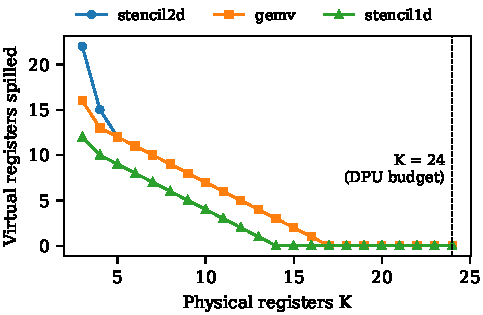
\includegraphics[width=\columnwidth]{figures/fig_spills.pdf}
\caption{Metric 5: virtual registers spilled by the Chaitin--Briggs allocator as the register budget $K$ varies.}
\label{fig:spills}
\end{figure}

\subsection{Metric 6: Compile Time}
Fig.~\ref{fig:compile} shows the time to compile each benchmark from source to DPU assembly and host C (median of seven runs). The mean is 42.1\,ms and the maximum 59.9\,ms (stencil2d). The rejected kernels compile in 18--23\,ms because no DPU code is generated for them. The analyses behind the decision, including footprint enumeration and the enumeration of direction vectors, therefore add negligible cost to compilation.

\begin{figure}[!t]
\centering
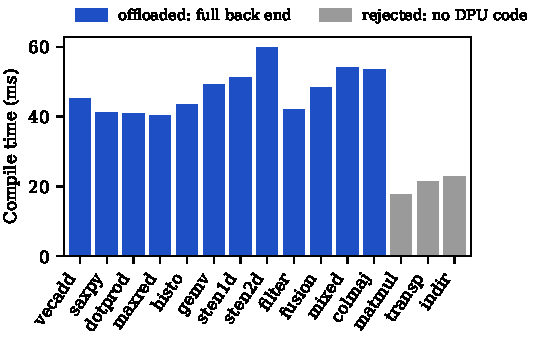
\includegraphics[width=\columnwidth]{figures/fig_compile.pdf}
\caption{Metric 6: compile time per benchmark, from source to generated code (median of seven runs).}
\label{fig:compile}
\end{figure}

\subsection{Ablation of the Decision Checks}
To see whether every check of (\ref{eq:predicate}) earns its place, we removed each in turn and asked which verdict would change and with what effect, using the failed-check lists that Algorithm~\ref{alg:decide} records and the simulated times of the affected programs. Table~\ref{tab:ablation} gives the outcome. Removing the arithmetic-intensity check or the reuse check alone changes no verdict on this suite, because matrix multiplication fails three checks and either of the remaining two still rejects it; the checks overlap deliberately, so that a compute-bound kernel is caught for more than one reason. The reuse threshold matters in the other direction: a literal rule that forbids any self-temporal reuse would reject gemv and lose its 1.29$\times$ speedup. The irregularity, partitioning and size checks each prevent a real loss, and the parallelism check prevents a wrong result rather than a slow one, since it is the only guard against running the iterations of a recurrence concurrently. The size check was motivated by a 256-element element-wise loop (\texttt{tests/tiny\_size.nmc}) that passes every other check; the host finishes it in 7,428 simulated cycles, while blind offloading needs 128,383 (0.06$\times$), because the 80,000-cycle launch alone exceeds the host's total time. With the check, the compiler estimates 5,760 host cycles against a fixed PIM cost of 81,024 and keeps the loop on the host.

\begin{table}[!t]
\caption{Ablation: the effect of removing one check of the decision predicate.}
\label{tab:ablation}
\setlength{\tabcolsep}{2.5pt}
\renewcommand{\arraystretch}{1.1}
\centering
\begin{tabular}{|p{2.3cm}|p{2.6cm}|p{2.6cm}|}
\hline
\textbf{Check removed} & \textbf{Verdict that changes} & \textbf{Effect} \\ \hline
AI $<0.5$ & none (matmul still fails reuse and size) & -- \\ \hline
Significant reuse & none (matmul still fails AI and size) & -- \\ \hline
Threshold $\rho$ (any reuse rejects) & gemv rejected & 1.29$\times$ lost \\ \hline
Parallel outer loop & serial recurrences offloaded & wrong results (by construction; not simulated) \\ \hline
Not IRREGULAR & indirect offloaded & 1.00$\times\rightarrow$0.43$\times$ \\ \hline
Partitionable & transpose offloaded & 1.00$\times\rightarrow$0.70$\times$ \\ \hline
Size check & 256-element loop offloaded & 1.00$\times\rightarrow$0.06$\times$ \\ \hline
\end{tabular}
\end{table}

\subsection{Correctness}
All 45 benchmark--configuration runs produce results bit-identical to HOST\_ONLY, the unoptimised IR gives the same results as the optimised IR for every benchmark, and the generated, register-allocated DPU programs of all fifteen benchmarks execute with identical results in the interpreter. The test suite of eight programs and 365 checks passes, and the simulator's dynamic coherence checker reports no stale read. The last property also shows that the slowdowns of blind offloading are performance effects, not errors.

\subsection{Discussion and Limitations}
The results support the central claim that near-memory offloading should be conditional and that a small set of classical analyses is enough to make the condition reliable on this benchmark set. The most instructive cases are the three rejections, because each fails for a different reason that a single metric cannot see. Matrix multiplication is parallel and would be accepted by a parallelism-only rule, yet it is compute-bound and its working set fits the host cache. Transpose has an arithmetic intensity of zero and would be accepted by a roofline rule, yet its writes cross every partition. Indirect access looks memory-bound too, yet its subscripts are unknown at compile time, so every DPU would need a full copy of the indexed array. The predicate rejects all three, and the explanation it prints names the failing check in each case, which makes the decision easy to audit.

\emph{Threats to validity.} Construct validity depends on the simulator: cycles, bytes and energy are model outputs, and their relation to real hardware rests on the constants of Table~\ref{tab:params}. Internal validity is helped by determinism, since every run of the same program gives the same numbers and \texttt{make run-all} reproduces the published CSV exactly, but the per-benchmark values are single deterministic runs rather than measurements with variance. External validity is limited by the benchmark set, which contains fifteen small, single-kernel programs chosen to exercise each check; larger applications with several interacting kernels may behave differently. Conclusion validity is supported by the comparison of policies on the same simulator and the same inputs, so the relative ordering of the policies does not depend on the absolute calibration.

Several further limitations qualify the claim. The results come from a simulator, not from physical UPMEM hardware, and the constants of Table~\ref{tab:params} were chosen to be plausible rather than calibrated; the launch overhead and the per-run DMA cost have the largest influence on small kernels. The cost model optimises time and ignores energy, so it rejects transpose although offloading it would save energy. Data are copied in and out on every launch; keeping arrays resident across kernels would change several verdicts. Finally, the benchmarks are small, single-kernel programs; fusion currently requires both loops to use the same index variable, and fission refuses loops that contain strength-reduced accumulators.

% =============================================================================
\section{Conclusion and Scope for Future Work}
\label{sec:conclusion}
% =============================================================================

This paper presented NEMO-C, a compiler that decides for every loop nest whether it should run on the host or on processing-in-memory DPUs, and that refuses offloads which would make the program slower.

Existing PIM tools characterise the hardware or generate efficient PIM code, but they mostly leave the decision of what to offload to the programmer or confine it to neural-network operators.

NEMO-C makes the decision statically with six checks built from classical analyses, explains every verdict, and uses fission, interchange and fusion to turn rejected loops into profitable ones.

It is implemented from scratch in C++17 with Flex and Bison and evaluated in a cycle-level simulator of an UPMEM-style system.

On fifteen benchmarks NEMO-C is never slower than the host and reaches a geometric-mean speedup of 1.42$\times$ and a best case of 7.47$\times$. It avoids the 0.63$\times$, 0.70$\times$ and 0.43$\times$ slowdowns of blind offloading and makes the correct decision on all fifteen benchmarks, against twelve for an arithmetic-intensity-only rule. It reduces memory-bus traffic to 0.67$\times$ and energy to 0.70$\times$ of the host's, and every one of its 45 simulated runs, including the execution of its own generated assembly, is bit-identical.

Future work will first calibrate the cost model against measurements on real UPMEM hardware and study the sensitivity of the verdicts to the launch and transfer constants. The decision should become energy-aware, so that a user can trade time for energy. Keeping arrays resident in PIM across kernel calls, and deciding offloads for whole programs rather than isolated nests, would extend the approach to multi-kernel applications. Support for irregular loops, for example by partial offload with inspector--executor techniques, and an exact integer dependence test would widen the set of loops the compiler can accept.

% =============================================================================
\section*{Author Contributions}
% =============================================================================
Somesh Tripathi conceived the project, designed and implemented the complete NEMO-C compiler (front end, intermediate representation and classical optimisations, dependence analysis, offload cost model, loop transformations, partitioning and coherence, code generation and register allocation), the simulator, the test suite and the browser workbench, ran all experiments and analysed the results. Somesh Tripathi, Smeehen and Swati Saumya contributed to the literature survey and to writing, editing and reviewing the manuscript. All authors read and approved the final manuscript.

\section*{Acknowledgment}
The authors thank the School of Computer Science and Engineering, Vellore Institute of Technology, for the resources provided for this Compiler Design project. The AI assistant Claude (Anthropic), used through Claude Code, assisted in this work: it helped write, debug and test parts of the compiler, and also helped with parts of the text, figures and LaTeX source of this manuscript. The authors directed this use, checked every number in the paper against the compiler's own output in \texttt{results/results.csv}, verified the cited works, and take full responsibility for the content.

\section*{Funding}
This research received no specific grant from any funding agency in the public, commercial, or not-for-profit sectors.

\section*{Competing Interests}
The authors declare no competing financial or non-financial interests.

\section*{Data and Code Availability}
The complete source code of NEMO-C, the fifteen benchmark programs, the test suite, the simulation results and the scripts that produce every figure of this paper are available at \url{https://github.com/Somesh2223/Near-Memory-Computing-Compiler}.

% =============================================================================
% References, numbered in order of first citation, in the format required by
% the course template.
% =============================================================================
\begin{thebibliography}{00}

\bibitem{mutlu2019where} Mutlu, Onur, Saugata Ghose, Juan G\'omez-Luna, and Rachata Ausavarungnirun. (2019) ``Processing data where it makes sense: Enabling in-memory computation.'' \emph{Microprocessors and Microsystems} 67: 28--41.

\bibitem{singh2019nmc} Singh, Gagandeep, Lorenzo Chelini, Stefano Corda, Ahsan Javed Awan, Sander Stuijk, Roel Jordans, Henk Corporaal, and Albert-Jan Boonstra. (2019) ``Near-memory computing: Past, present, and future.'' \emph{Microprocessors and Microsystems} 71: 102868.

\bibitem{mutlu2020primer} Mutlu, Onur, Saugata Ghose, Juan G\'omez-Luna, and Rachata Ausavarungnirun. (2020) ``A modern primer on processing in memory.'' \emph{arXiv preprint} arXiv:2012.03112.

\bibitem{devaux2019upmem} Devaux, Fabrice. (2019) ``The true processing in memory accelerator.'' In \emph{Proceedings of the IEEE Hot Chips 31 Symposium (HCS)}, Stanford, CA, USA.

\bibitem{kwon2021fimdram} Kwon, Young-Cheon, \emph{et al.} (2021) ``25.4 A 20nm 6GB function-in-memory DRAM, based on HBM2 with a 1.2TFLOPS programmable computing unit using bank-level parallelism, for machine learning applications.'' In \emph{Proceedings of the IEEE International Solid-State Circuits Conference (ISSCC)}: 350--352.

\bibitem{ghose2019workload} Ghose, Saugata, Amirali Boroumand, Jeremie S. Kim, Juan G\'omez-Luna, and Onur Mutlu. (2019) ``Processing-in-memory: A workload-driven perspective.'' \emph{IBM Journal of Research and Development} 63 (6): 3:1--3:19.

\bibitem{boroumand2018google} Boroumand, Amirali, \emph{et al.} (2018) ``Google workloads for consumer devices: Mitigating data movement bottlenecks.'' In \emph{Proceedings of the 23rd International Conference on Architectural Support for Programming Languages and Operating Systems (ASPLOS)}: 316--331.

\bibitem{oliveira2022methodologies} Oliveira, Geraldo F., Juan G\'omez-Luna, Saugata Ghose, and Onur Mutlu. (2022) ``Methodologies, workloads, and tools for processing-in-memory: Enabling the adoption of data-centric architectures.'' In \emph{Proceedings of the IEEE Computer Society Annual Symposium on VLSI (ISVLSI)}; \emph{arXiv preprint} arXiv:2205.14647.

\bibitem{gomezluna2023ml} G\'omez-Luna, Juan, Yuxin Guo, Sylvan Brocard, Julien Legriel, Remy Cimadomo, Geraldo F. Oliveira, Gagandeep Singh, and Onur Mutlu. (2023) ``Evaluating machine learning workloads on memory-centric computing systems.'' In \emph{Proceedings of the IEEE International Symposium on Performance Analysis of Systems and Software (ISPASS)}, doi:10.1109/ISPASS57527.2023.00013.

\bibitem{item2023transpimlib} Item, Maurus, Juan G\'omez-Luna, Yuxin Guo, Geraldo F. Oliveira, Mohammad Sadrosadati, and Onur Mutlu. (2023) ``TransPimLib: Efficient transcendental functions for processing-in-memory systems.'' In \emph{Proceedings of the IEEE International Symposium on Performance Analysis of Systems and Software (ISPASS)}: 235--247.

\bibitem{ke2020recnmp} Ke, Liu, \emph{et al.} (2020) ``RecNMP: Accelerating personalized recommendation with near-memory processing.'' In \emph{Proceedings of the ACM/IEEE 47th Annual International Symposium on Computer Architecture (ISCA)}; \emph{arXiv preprint} arXiv:1912.12953.

\bibitem{cooper2022engineering} Cooper, Keith D., and Linda Torczon. (2022) \emph{Engineering a Compiler}, 3rd edition. Cambridge, MA, USA: Morgan Kaufmann.

\bibitem{gomezluna2022prim} G\'omez-Luna, Juan, Izzat El Hajj, Ivan Fernandez, Christina Giannoula, Geraldo F. Oliveira, and Onur Mutlu. (2022) ``Benchmarking a new paradigm: Experimental analysis and characterization of a real processing-in-memory system.'' \emph{IEEE Access} 10: 52565--52608.

\bibitem{devic2022topim} Devic, Alexandar, Siddhartha Balakrishna Rai, Anand Sivasubramaniam, Ameen Akel, Sean Eilert, and Justin Eno. (2022) ``To PIM or not for emerging general purpose processing in DDR memory systems.'' In \emph{Proceedings of the 49th Annual International Symposium on Computer Architecture (ISCA)}: 231--244.

\bibitem{khan2023cinm} Khan, Asif Ali, Hamid Farzaneh, Karl F. A. Friebel, Cl\'ement Fournier, Lorenzo Chelini, and Jeronimo Castrillon. (2023) ``CINM (Cinnamon): A compilation infrastructure for heterogeneous compute in-memory and compute near-memory paradigms.'' \emph{arXiv preprint} arXiv:2301.07486.

\bibitem{chen2023simplepim} Chen, Jinfan, Juan G\'omez-Luna, Izzat El Hajj, Yuxin Guo, and Onur Mutlu. (2023) ``SimplePIM: A software framework for productive and efficient processing-in-memory.'' In \emph{Proceedings of the 32nd International Conference on Parallel Architectures and Compilation Techniques (PACT)}: 99--111.

\bibitem{oliveira2023dappa} Oliveira, Geraldo F., Alain Kohli, David Novo, Juan G\'omez-Luna, and Onur Mutlu. (2023) ``DaPPA: A data-parallel programming framework for processing-in-memory architectures.'' \emph{arXiv preprint} arXiv:2310.10168.

\bibitem{shin2023pimflow} Shin, Yongwon, Juseong Park, Sungjun Cho, and Hyojin Sung. (2023) ``PIMFlow: Compiler and runtime support for CNN models on processing-in-memory DRAM.'' In \emph{Proceedings of the 21st ACM/IEEE International Symposium on Code Generation and Optimization (CGO)}: 249--262.

\bibitem{oliveira2021damov} Oliveira, Geraldo F., Juan G\'omez-Luna, Lois Orosa, Saugata Ghose, Nandita Vijaykumar, Ivan Fernandez, Mohammad Sadrosadati, and Onur Mutlu. (2021) ``DAMOV: A new methodology and benchmark suite for evaluating data movement bottlenecks.'' \emph{IEEE Access} 9; \emph{arXiv preprint} arXiv:2105.03725.

\bibitem{giannoula2022sparsep} Giannoula, Christina, Ivan Fernandez, Juan G\'omez-Luna, Nectarios Koziris, Georgios Goumas, and Onur Mutlu. (2022) ``SparseP: Towards efficient sparse matrix vector multiplication on real processing-in-memory architectures.'' \emph{Proceedings of the ACM on Measurement and Analysis of Computing Systems} 6 (1): Article 21.

\bibitem{boroumand2019conda} Boroumand, Amirali, Saugata Ghose, Minesh Patel, Hasan Hassan, Brandon Lucia, Rachata Ausavarungnirun, Kevin Hsieh, Nastaran Hajinazar, Krishna T. Malladi, Hongzhong Zheng, and Onur Mutlu. (2019) ``CoNDA: Efficient cache coherence support for near-data accelerators.'' In \emph{Proceedings of the 46th International Symposium on Computer Architecture (ISCA)}: 629--642.

\bibitem{wang2023infinity} Wang, Zhengrong, Christopher Liu, Aman Arora, Lizy John, and Tony Nowatzki. (2023) ``Infinity Stream: Portable and programmer-friendly in-/near-memory fusion.'' In \emph{Proceedings of the 28th ACM International Conference on Architectural Support for Programming Languages and Operating Systems (ASPLOS), Volume 3}: 359--375.

\bibitem{oliveira2024mimdram} Oliveira, Geraldo F., Ataberk Olgun, Abdullah Giray Ya\u{g}l{\i}k\c{c}{\i}, F. Nisa Bostanc{\i}, Juan G\'omez-Luna, Saugata Ghose, and Onur Mutlu. (2024) ``MIMDRAM: An end-to-end processing-using-DRAM system for high-throughput, energy-efficient and programmer-transparent multiple-instruction multiple-data computing.'' In \emph{Proceedings of the IEEE International Symposium on High-Performance Computer Architecture (HPCA)}: 186--203.

\bibitem{hajinazar2021simdram} Hajinazar, Nastaran, Geraldo F. Oliveira, Sven Gregorio, Jo\~ao Dinis Ferreira, Nika Mansouri Ghiasi, Minesh Patel, Mohammed Alser, Saugata Ghose, Juan G\'omez-Luna, and Onur Mutlu. (2021) ``SIMDRAM: A framework for bit-serial SIMD processing using DRAM.'' In \emph{Proceedings of the 26th ACM International Conference on Architectural Support for Programming Languages and Operating Systems (ASPLOS)}, doi:10.1145/3445814.3446749.

\bibitem{lee2021hbmpim} Lee, Sukhan, \emph{et al.} (2021) ``Hardware architecture and software stack for PIM based on commercial DRAM technology: Industrial product.'' In \emph{Proceedings of the ACM/IEEE 48th Annual International Symposium on Computer Architecture (ISCA)}: 43--56.

\bibitem{hyun2024pathfinding} Hyun, Bongjoon, Taehun Kim, Dongjae Lee, and Minsoo Rhu. (2024) ``Pathfinding future PIM architectures by demystifying a commercial PIM technology.'' In \emph{Proceedings of the IEEE International Symposium on High-Performance Computer Architecture (HPCA)}: 263--279.

\bibitem{sun2023pimcomp} Sun, Xiaotian, \emph{et al.} (2023) ``PIMCOMP: A universal compilation framework for crossbar-based PIM DNN accelerators.'' In \emph{Proceedings of the 60th ACM/IEEE Design Automation Conference (DAC)}; \emph{arXiv preprint} arXiv:2307.01475.

\bibitem{bison2021manual} Free Software Foundation. (2021) ``GNU Bison: The Yacc-compatible parser generator, version 3.8.'' Available: \url{https://www.gnu.org/software/bison/manual/}.

\bibitem{gcc2024manual} Free Software Foundation. (2024) ``Using the GNU Compiler Collection (GCC).'' Available: \url{https://gcc.gnu.org/onlinedocs/}.

\bibitem{matplotlib2024} The Matplotlib Development Team. (2024) ``Matplotlib: Visualization with Python.'' Available: \url{https://matplotlib.org/}.

\end{thebibliography}

\EOD

\end{document}
